\chapter{CERN, the LHC and LHCb}
\label{CERN_LHC_LHCb}

The European Organisation for Nuclear Research (CERN) was founded in 1954, ot began with 12 member states as a organisation to encourage European collaboration and the study of nuclear physics. The collaborative nature of CERN allowed large-scale expensive experiments to be built that individual member states would not have be able to create. The Proton Synchrotron (PS) was CERN's flagship accelerator, operational in 1959 it had a circumference of 628~m and accelerated protons to 25~\gev. The PS was the the highest energy particle accelerator at that time. Now 62 years since it's foundation, CERN has grown to include 22 member states~\footnote{Countries and organisations that are unable to become member states can still particlipate in scientific research as obserser states \cite{Member_States}.} and is still at the forefront of high energy physics research. CERN’s latest accelerator, the Large Hadron Collider (LHC), is most energetic particle accelerator ever built, with a 27~km circumference the LHC was designed to protons at 14~\tev. This chapter shall discuss the LHC and the LHC beauty experiment, one of the experiments that studies particle collisions provided by the LHC.

\section{The LHC}
\label{LHC}


The LHC is a proton synchrotron designed to accelerate and collide two beams of protons with a center-of-mass energy of 14~\tev. Although operation of the LHC began in 2010 it is yet to reach the design center of mass energy. The purpose of the LHC is to provide high energy proton collisions, the products of which are used for precision tests of the Standard Model (SM) and to search for new physics particles that go beyond the scope of the SM. There are four interaction points on the LHC ring where the beams are brought to collide, at these points various experiments detect and study the products of these collisions. The LHC can also accelerate lead-nuclei up to 2.76~\tev per nucleon, it is only the products from proton collisions that are relevant for the topic of this thesis.

%It's the bit below that I'm not a massive fan of the explains how the LHC gets it's protons. I think that it is a little too brief and disconnected with not explanations.
The protons for the LHC come from hydrogen gas, %add something nice here
the hydrogen atoms are ionised to strip away the electrons and the protons are accelerated through a chain of particle accelerators of increasing energy before being injected into the LHC. The chain of accelerators, shown in Fig.~\ref{fig:accelerator_chain}, consists of accelerators that were used in experiments throughout the second half of the last century and have been modified to meet the requirements needed to provide protons for the LHC. 
\begin{figure}[htbp!]
  \centering
  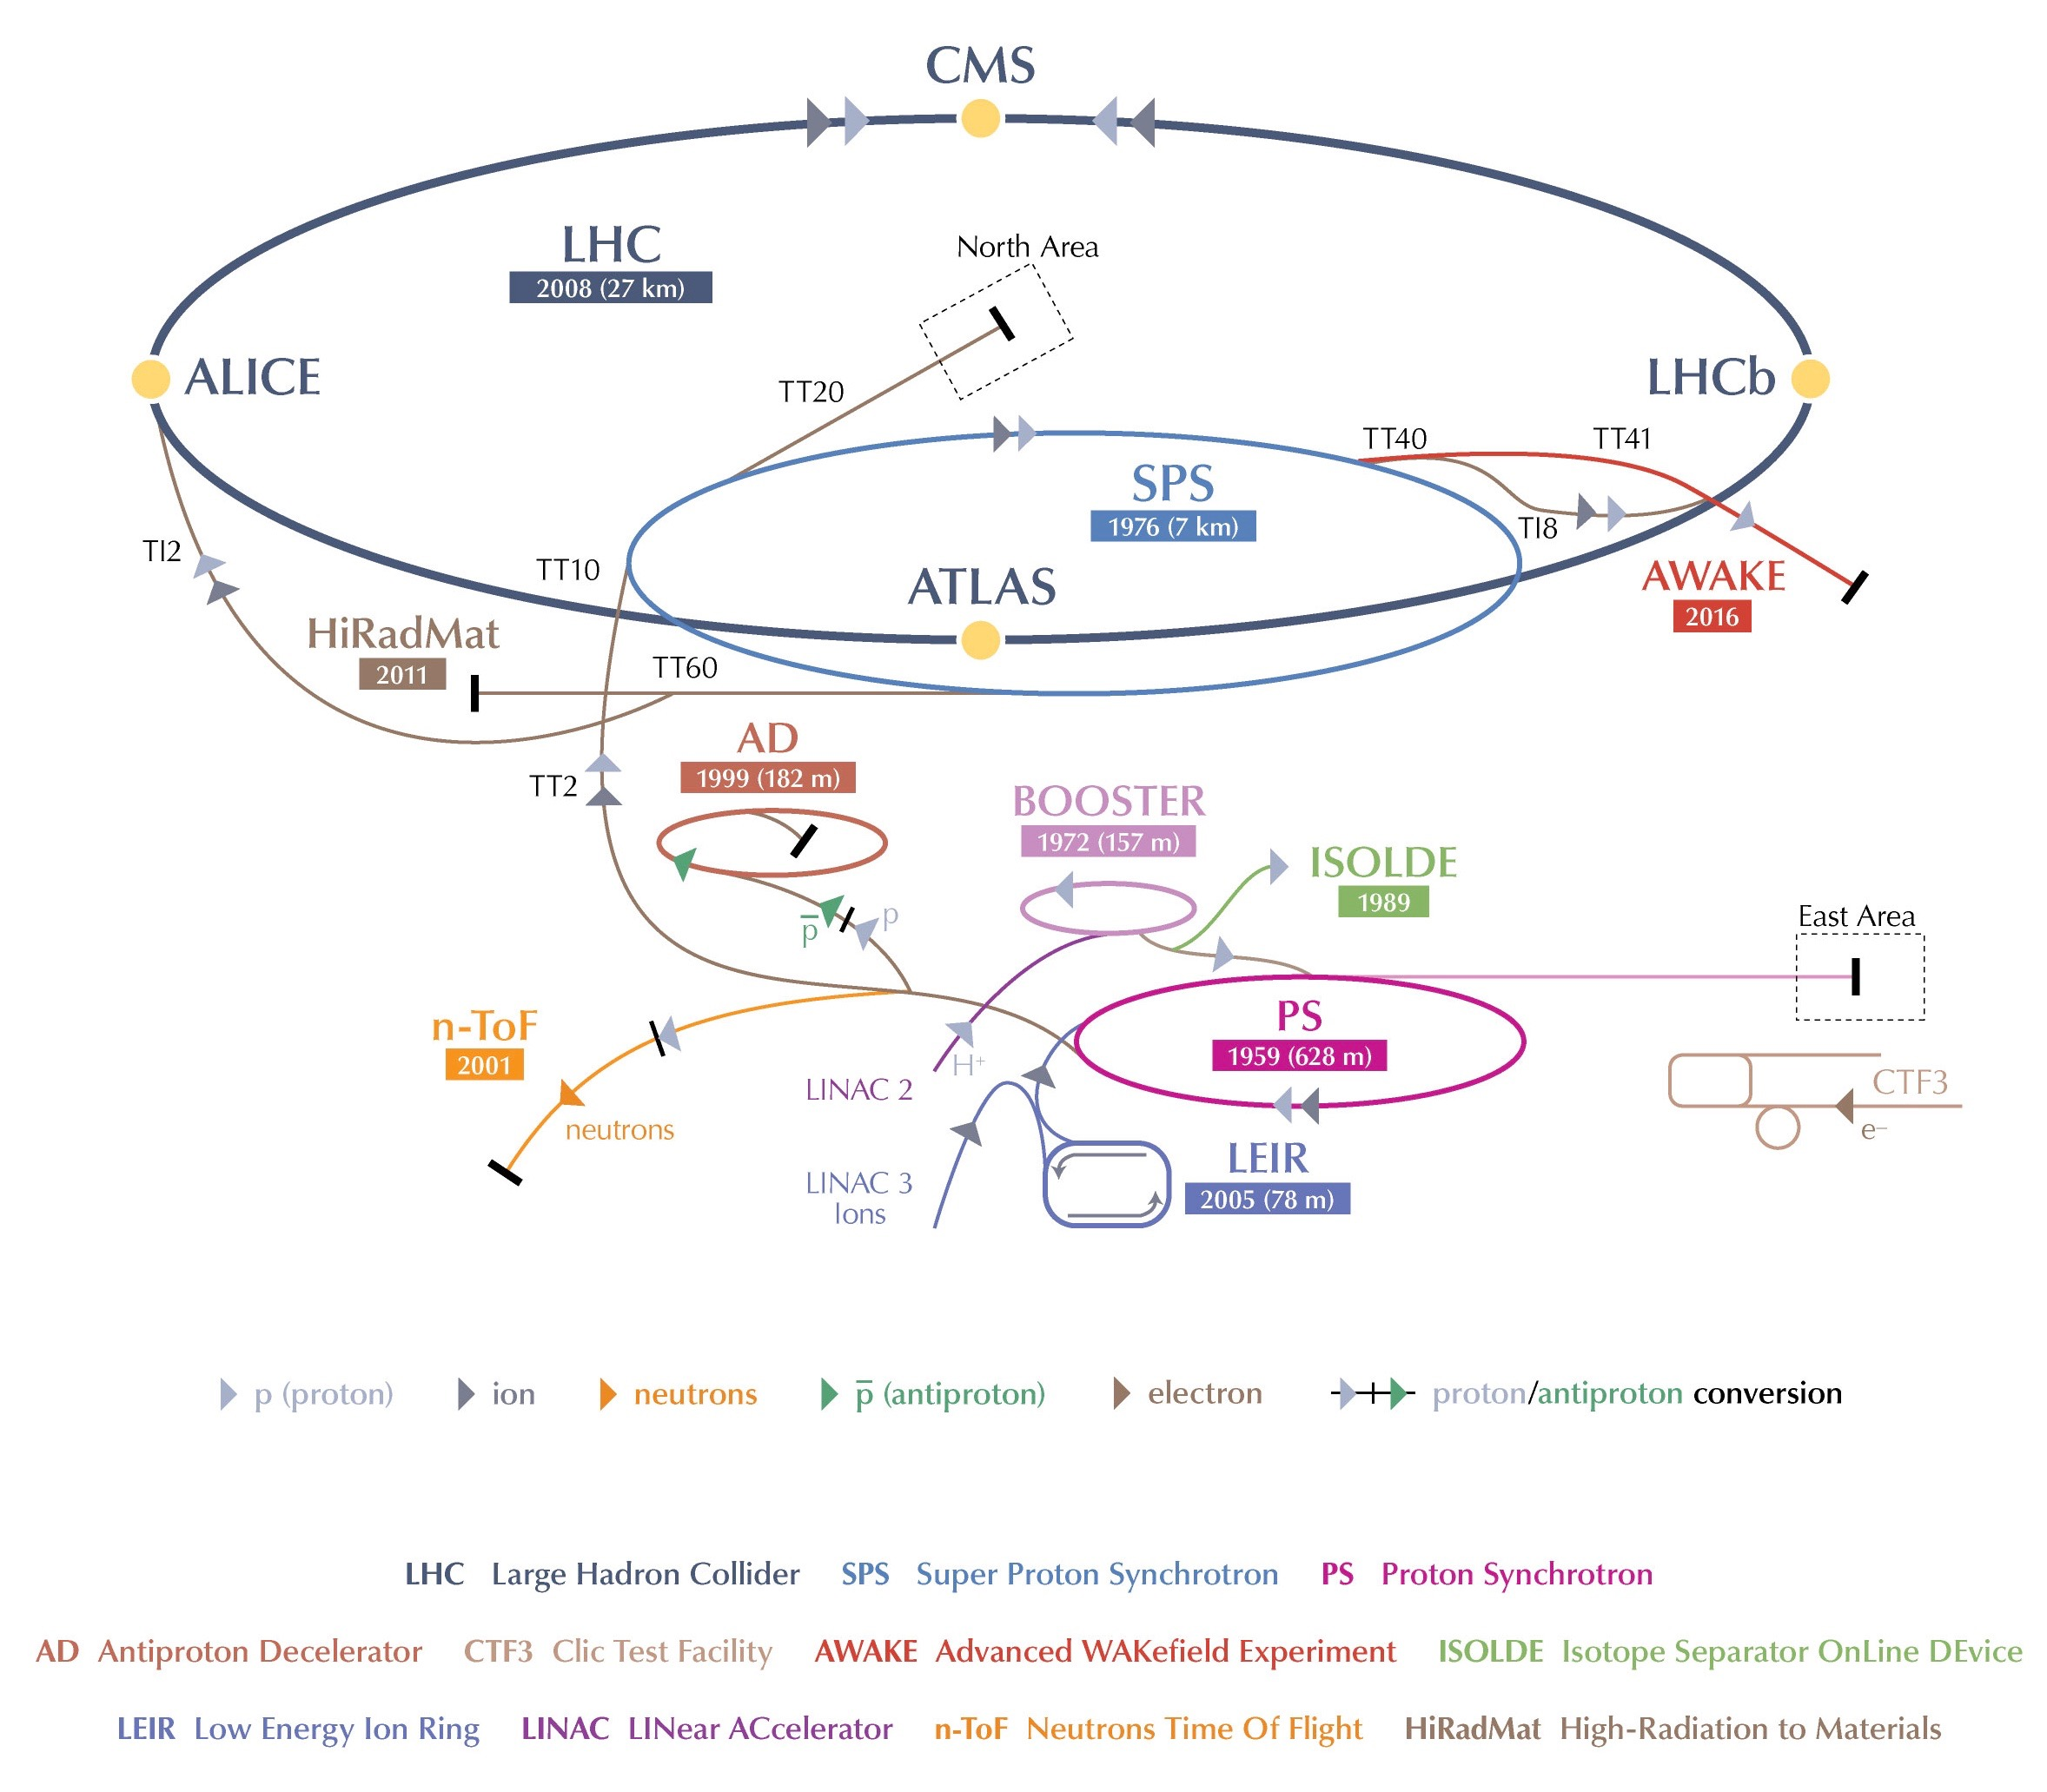
\includegraphics[trim = 125mm 2mm 125mm 90mm, clip, width=0.8\textwidth]{./Figs/LHC_LHCb/accelerator_complex.jpg}
  \caption{The accelerator complex at CERN. The chain of accelerators used to inject protons into the LHC begins with the Linac 2 which accelerates pr\
otons to 50~\mev, these are passed to the Proton Synchrotron Booster that accelerates the protons to 1.4 \gev. The Proton Synchrotron is next in the chain, accelerating protons to 25~\gev and cre\
ating the desired spacing between proton bunches. Then finally the Super Proton Synchrotron accelerating protons to 450~\gev ready for injection into the LHC. Source: CERN.}
  \label{fig:accelerator_chain}
\end{figure}



The protons leave the chain of accelerators with of energy of 450~\gev per proton and in bunches of \~$10^{11}$ protons, as the bunches are injected into the LHC they are split into two oppositely circulating beams.
The LHC accelerates the protons to the desired center of mass energy using supercooled radio frequency cavities and guides them around the ring with superconducting dipole magnets. %I could add here some details about the magnets and how the LHC accelerates the protons.
Once the required energy has been reached, the bunches are focused using quadrupole magnets before being brought to collided at 4 interaction points around the LHC ring.% at a bunch crossing rate of 40~MHz. 

The center of mass energy of a collider is an important measure of its performance as it dictates what particles could be produced in collisions, another important measure of collider performance is the instantaneous luminosity a collider can provide. The instantaneous luminosity, $\mathcal{L}$, is a measure of how many collision occur per second, it is given by

\begin{equation}
\mathcal{L} = \frac{N^{2} f n_{b}}{\mathcal{F}}.
\label{eq:inst_lumi}
\end{equation}


where $N$ is the number of protons per bunch, $n_{b}$ the number of bunches per beam, $f$ the bunch revolution frequency and $\mathcal{F}$ contains information about the beam geometry. The LHC is designed to operate at a maximum instantaneous luminosity of $10^{34}$~cm$^{-2}$s$^{-1}$. To reach this luminosity the LHC can have up to 2808 proton bunches per beam with a revolution frequency if the beams at 11.245 kHz, therefore the separation between proton bunches can be as short as 25~ns. The higher the luminosity, the more collisions happen in a second and the more particles will be produced, this can either be advantageous or disadvantageous depending on the physics process that is being studied.
% and the detector design that records the collisions. 
Therefore luminosity delivered at each interaction point can be tuned by the quadrupole magnets by altering the shape of each bunch to suit the experiments at each point.

Proton beams first circulated the LHC in 2008 and since then there have been two physics runs separated by a long shutdown period. Run 1 began in 2010 and continued until 2013, during this time protons were collided with a center of mass energy of $\sqrt{s}$ = 7~TeV in 2010 and 2011 then this energy was increased to $\sqrt{s}$ =8~TeV for 2012. After Run~1 came first long shutdown (LS1), during this time work was done to prepare the LHC to operate at higher energies and renovation work was preformed on accelerators that provide the LHC with protons. Run~2 began in 2015 with proton collisions at a center of mass energy of $\sqrt{s}$ =  13~TeV, %why 13TeV? I have the answer
this Run will continue until 2018 when a second period of upgrades and maintenance, the Long Shutdown~2, will begin.




There are 7 experiments on the LHC that detect particles produced in proton and heavy ion collisions. There are two general purpose detectors, ATLAS and CMS, that were designed to search for the Higgs boson and new particles that are beyond the scope of the SM in proton collisions, these two experiments operate at the full instantaneous luminosity of the LHC. %Perhaps say we found the Higgs?
ALICE studies quark-gluon plasma produced in heavy ions collisions to understand conditions similar to those present in the early universe. The TOTEM experiment studies properties of protons as they collide head on at the LHC and the MOEDAL experiment is aims to detect magnetic monopoles. The LHCf experiment is a very forward experiment studying particles that are thrown forward in LHC collisions to understand similar processes that occurrs in cosmic rays. Finally there is the Large Hadron Collider Beauty experiment (LHCb) that will be described in the next section. %, this experiment was designed to studies rare $b$-hadron decays and $\mathcal{CP}$ violating processes and operates at a lower luminosity and has a smaller angular acceptance than the general purpose detectors. %Should probably include the full experiment names as I have done for LHCb or not include the name for LHCb.




\section{LHCb Experiment}
\label{LHCb}
The LHCb experiment is one of the 7 experiments located on the Large Hadron Collider. It was built in order to search for indirect evidence of new physics phenomona through the study of CP violation and rare decays for hadrons that contain b and c quarks.

In proton collisions provided by the LHC heavy quark pairs are predominantly produced at small angles to the beam pipe. The dominant production mechanisms that produced bbbar pairs are quark anti-quark annihilation, gluon-gluon fusions and  gluon splitting as shown in the Feynman diagrams in Figure X. There must be some other reason why these processes lead to the quarks being boosted along the beam pipe and I shall explain that here. Once the bbbar pairs are produced the quarks hadronise(?), in to Bs, Bd, B+ and many others and the decays of these hadrons have some specific characteristics. B-mesons have long lifetime around 1 ps therefore travel ~1cm from the interaction vertex where they were produced before decaying at a secondary vertex. Good identification of the secondary vertices is necessary to determine that the B hadrons decay into. Since b quarks are heavy quarks, the hadrons they for can decay into a large range of differnt particles from light particle such as electrons and photons to heavier particles like kaons, muons and D meson. Therefore a good detector for b physics needs to be able to identity a range of decay produced to accurately reconstruct what actually decayed. The experiment was designed around the production characteristics of bbbar pairs and to enable precise measurements of b hadron decays. 

The LHCb experiment was built as a single arm forward spectrometer, with an angular coverage of 10 to 300 mrad in the vertical direction and 10 to 250 mrad in the horizontal direction relative the the beam pipe. This angular coverage what chosen to exploit the small angles relative the the beam pipe that bbbar pairs are produced at. A cross-section of the detector is shown in Figure \ref{fig:LHCb_detector}, where a right handed coordinate system is used. Protons collide at the interaction point on the left hand side of the diagram, the products of the collisions then travel through the detector leaving information in the different sub detectors along the length of the detector. The information deposited in the sub detectors are reconstructed to determine what happened in the proton collisions. The sub detectors can be classified in to two main categories; tracking system and particles identification system .

\begin{figure}[htb] 
  \centering    
  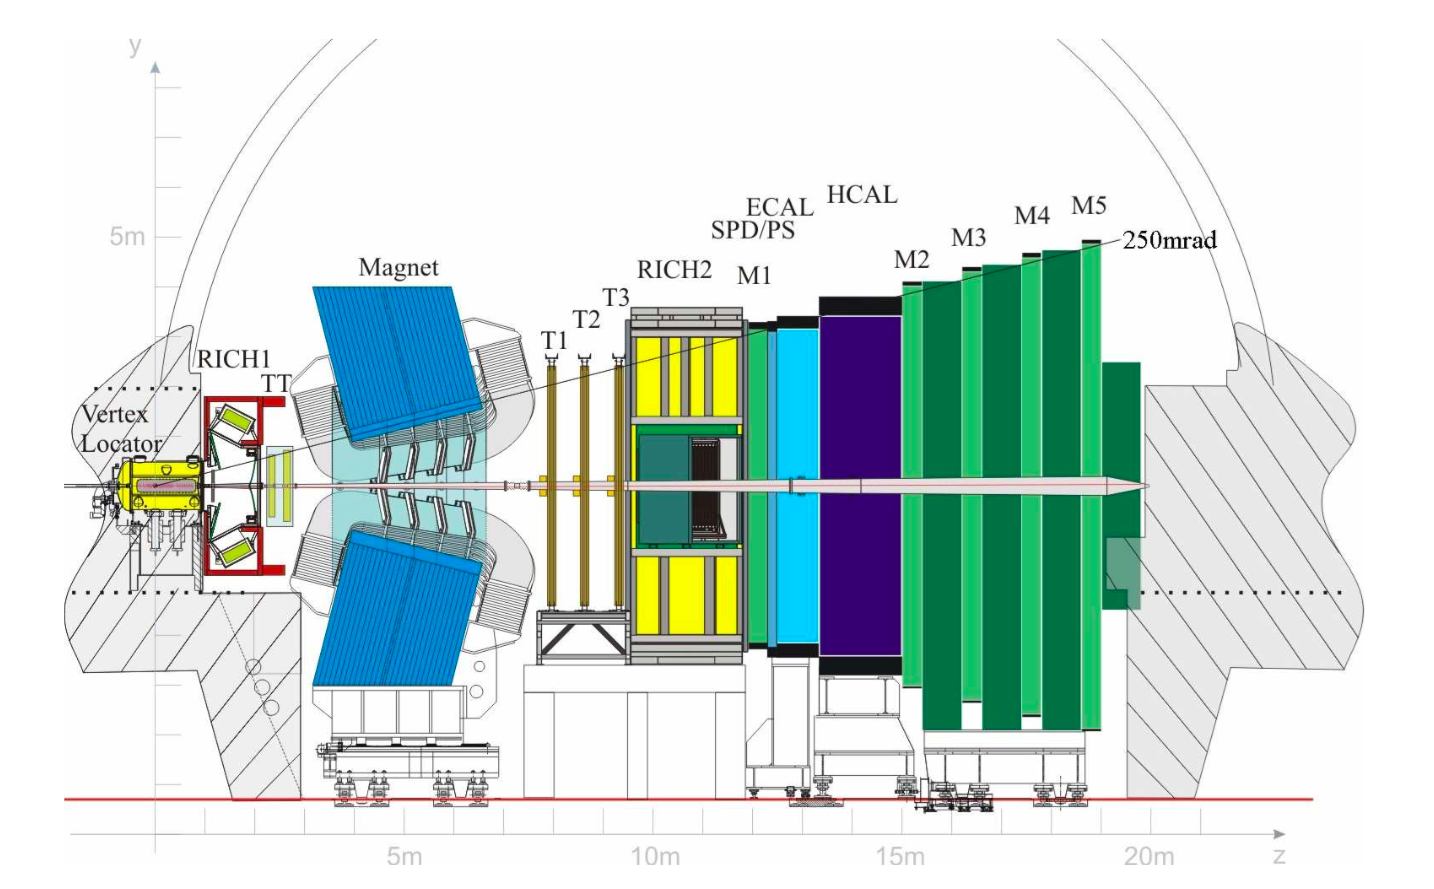
\includegraphics[ width=1.0\textwidth]{./Figs/LHC_LHCb/lhcb.png}
  \caption{Cross section of the LHCb detector \cite{Alves:2008zz}.}
  \label{fig:LHCb_detector}
\end{figure}

The tracking system is make up to the vertex locator (VELO), the magnet, the TT and the tracking stations T1-3. The VELO is designed to provide precise tracking measurements to identity the primary and secondary vertices characteristic of \bhadron decays in order to determine accurate lifetimes of \bhadrons. The magnet and tracking stations are combined to give high momentum resolution which is necessary to achieve good mass resolution which is used to distinguish between different b hadrons and separate signal and background decays.
%Need good decay time resolution if we are to measure the rapidly oscillatin Bs system.
The particle identification detectors provide complementary information about the identity of particles passing through them which enables the many different decay products of \bhadrons to be identified and the hadron to be accurately reconstructed. The RICH detectors provide information about these types of particles, the two calorimeters give informations that separates electrons, positrons and photons and from hadrons. Finally the muons stations at the furthest point from the integration point identify muons as the name suggests. 

The measurement of of decays of heavy hadrons requires accurate reconstruction of secondary vertices, this is achieved in part by the tracking systems however another aspect of the LHCb experiment deigns that enables this is the luminosity the experiment operates at. The LHC was designed to deliver a luminosity of X, proton collisions at this luminosity leads to a large amount of pile up. Pile up is stuff from the decay that is not interesting and is close to the beam pipe, therefore in the LHCb acceptance and makes it hard to accurately reconstruct secondary verticies. Therefore LHCb operates at a lower luminosity of ~ X in order to reduce the amount of pile up and enable accurate reconstruction of b hadron decays. 

The tracking and PID systems are described in the following sections as well as the way events are selected at LHCb and processed and analyses. 

%\begin{figure}[tb] 
%  \centering    
%  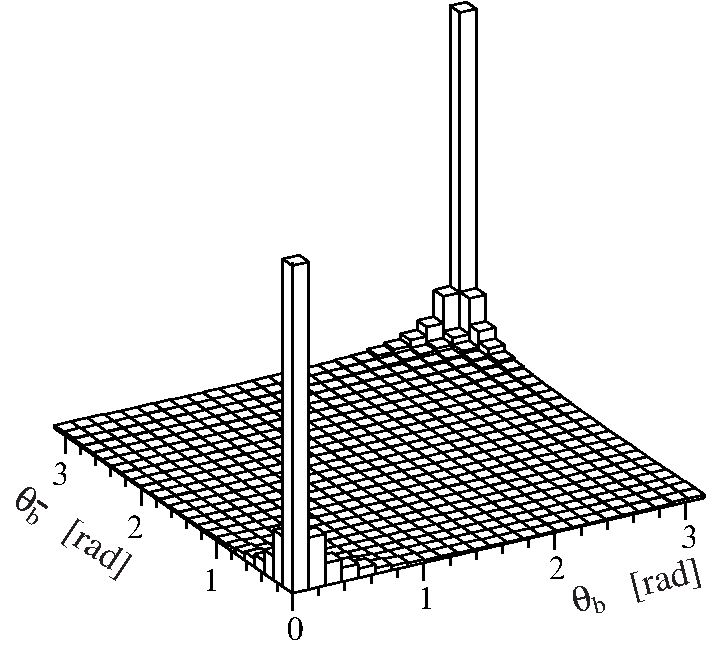
\includegraphics[ width=1.0\textwidth]{./Figs/LHC_LHCb/b_distrib_lhcb.pdf}
%  \caption{Simulated angular distribution for b-quark production at the LHC, angles are relative the the beam pipe with $\theta =0$ in the forward direction and$\theta = \pi$  in the backward direction \cite{Amato:1998xt}.}
%  \label{fig:LHCb_detector}
%\end{figure}


\subsection{Tracking}
\label{Tracking}

The tracking system within the LHCb experiment consists of the VELO, the magnet and the tracking stations which are the Tracker Turicensis (TT) and three tracking stations (T1-3). The VELO surrounds the interaction point and the magnet is between the TT and the tracking stations (T1-3). Together they work to provide precise information of the passage of charged particles though the detector which is needed for accurate analysis for \bhadron decays. The VELO gives precise information about the primary and secondary vertices where as the tracking stations give full track reconstruction. 

\subsubsection{VELO}
\label{VELO}
The VELO is a silicon detector that surrounds the interaction point. It’s main goal is to provide precise information about the interaction vertices and secondary decay vertices of particles produced in proton collisions. Important to give us lifetimes and impact parameters. The VELO covers the full LHCb angular acceptance.

The VELO is made up of 2 identical halves, each half consists of 21 stations each containing 2 silicon sensors arranged along the beam pipe. The arrangement is shown in figure \ref{fig:velo}. The z distribution is such that the flow covers the full LHCb acceptance and a charged track within the acceptance will pass through at least 3 stations. In each station the 2 sensor measure different coordinates, one measures the r coordinates of charged particles and the other measures the phi coordinates they are distributed along the length of the VELO. The r, phi and z cordidiates are used to reconstruct charged particle trajectories. Cylindrical coordinates were chosen to allow for fast reconstruction for particle trajectories in the VELO so that the can be used in the trigger. Figure \ref{fig:types_of_tracks} shows examples of the two types of sensor in the VELO. There is a small hole in the centre of the sensors to let the beam through.

\begin{figure}[htb] 
  \centering    
  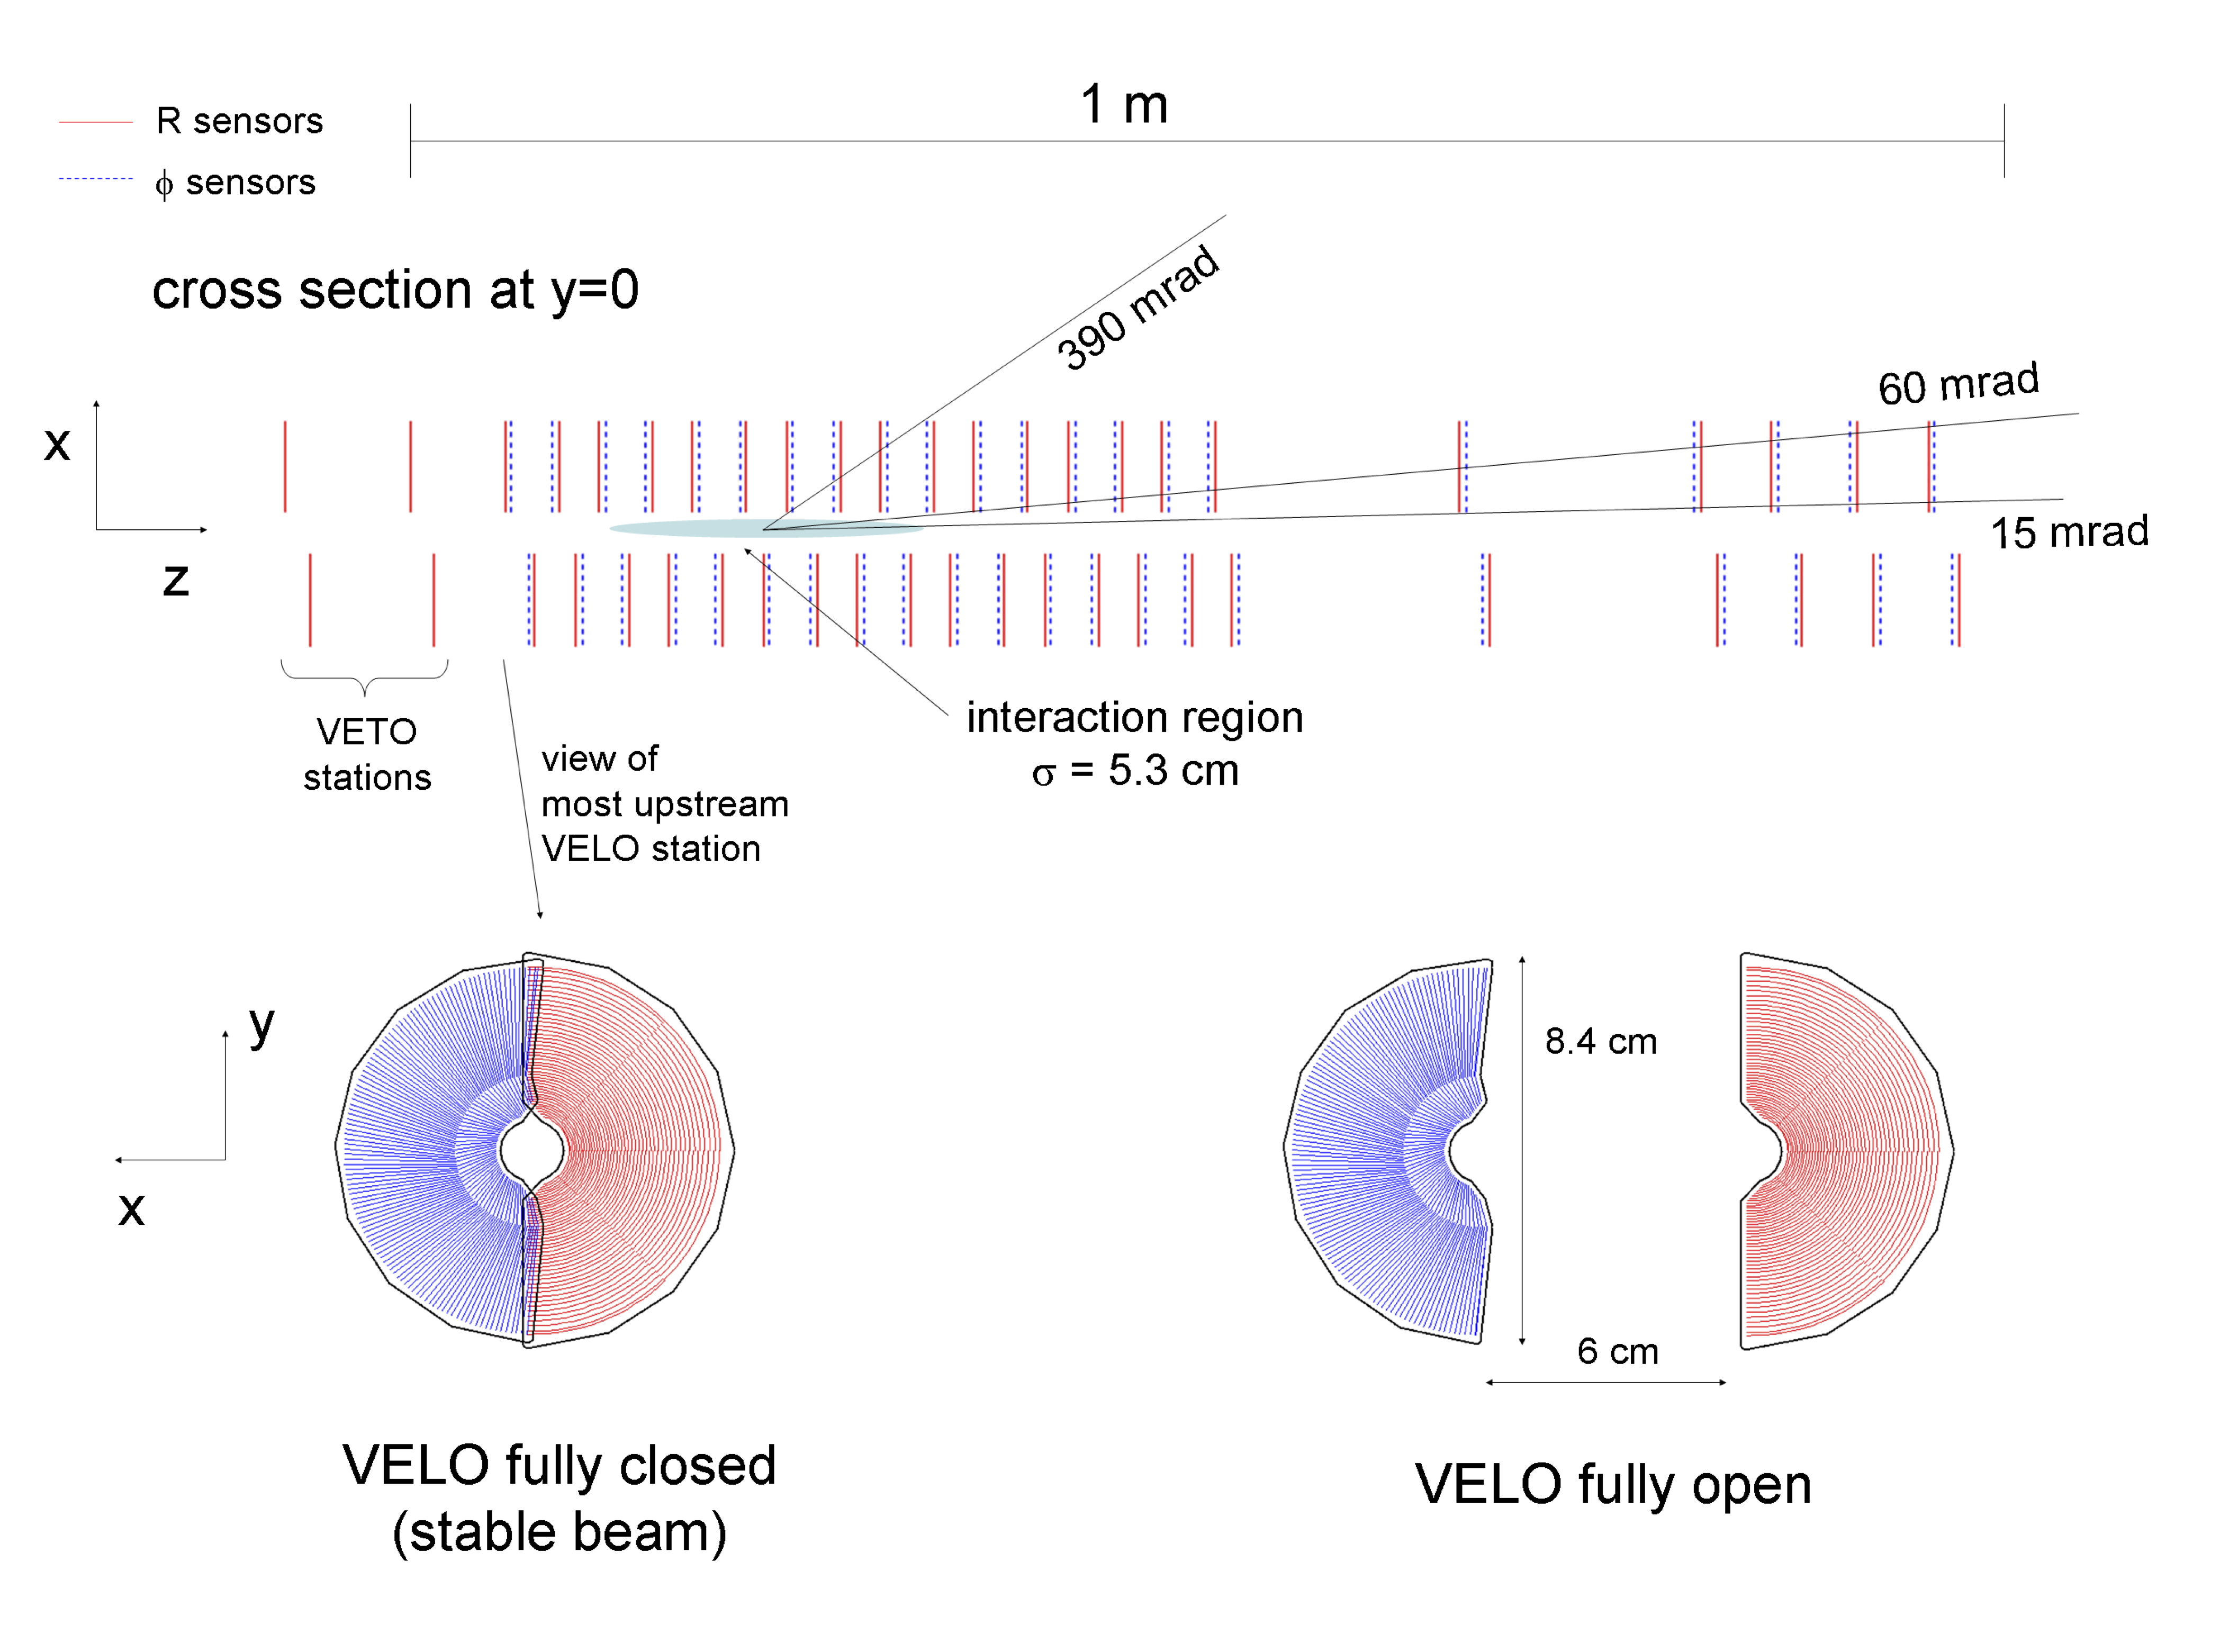
\includegraphics[ width=0.7\textwidth]{./Figs/LHC_LHCb/velo.png}
  \caption{The velo \cite{Alves:2008zz}.}
  \label{fig:velo}
\end{figure}

The momentum resolution of charged tracks depends on multiple scattering, therefore to allow for good momentum resolution to be determine in the other tracking stations, the VELO is kept in a vacuum so reduce it’s material budget. Each half of the VELO is enclosed inside an aluminium box, this keeps the VELO in a  vacuum the VELO but it also shields the electronic readouts of the VELO from radio frequencies which are generated by the beam. The VELO material budget comes to 17.5 $\%$ of a radiation length.

Excellent vertex resolution is required in the VELO, to achieve this the sensors in the VELO need to be as close as possible to the interaction point. This is achieve by having 2 separate halves to the VELO. During data taking when the VELO is record the location of primary and secondary vertices the veto sensor at only 8mm from the beam axis. However during the injection phase of the beam the width of the beam is much greater, therefore the 2 halves of the VELO can retract so that they are 3cm from the nominal beam axis which keeps them safe from radiation damage. This is all shown in Figure \ref{fig:velo}. The two half of the veto aren’t aligned, they are displaced by 150 mm in the z direction so that when the VELO is closed, the sensors in each half overlap, this helps with detector alignment and reduced edge effects. A photograph on one half of the VELO is shown in Figure  \ref{fig:velo_photo}.


\begin{figure}[htb] 
  \centering    
  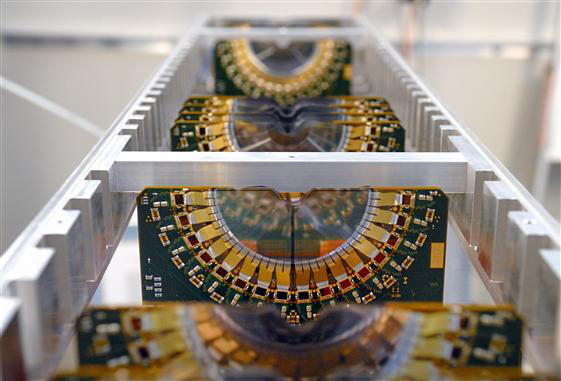
\includegraphics[ width=0.7\textwidth]{./Figs/LHC_LHCb/Velo_photo.jpg}% ./Figs/Detector/Velo_photo.jpg}
  \caption{The velo Soure: LHCb.}
  \label{fig:velo_photo}
\end{figure}

\begin{figure}[htb]
  \centering
  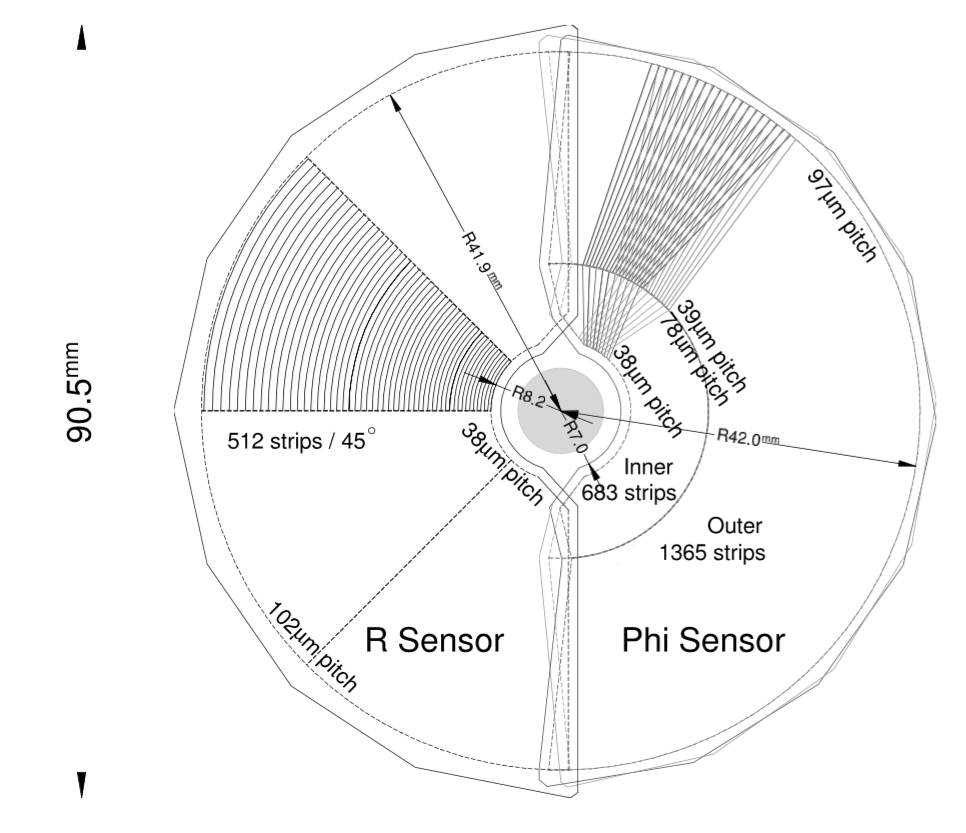
\includegraphics[ width=0.6\textwidth]{./Figs/LHC_LHCb/Velo_sensor_diagram.png}
  \caption{Velo sensor. Source: \cite{Alves:2008zz}.}
  \label{fig:types_of_tracks}
\end{figure}


Furthermore the interaction point is within the velo, there are sensors up stream of the interaction point which allows for accurate reconstruction of PVs.


Another feature if the VELO is that is can act a veto for high pile up events. There are 2 VELO sensor upstream of the interaction point that act a pile up vetoes, they given information to the trigger about how many pp interactions there were with each bunch crossing and help to select only what we’d be good a reconstructing. ( it rejects events with a large number of pp interactions)

Overall the VELO gives such and such precision.  vertex resolution in the transverse plane 10-20 mircons, in the z directions 50-100 microns depending on the number of tracks in the vertex. %The VELO is also important the impact parameter resolution and decay time resolutions.  (This may go at the end so that everything for tracking is together?) best resolution is 4 micrometers which allows a lifetime measurement of 50 fs. (Performance paper)



\subsubsection{Tracking Stations} 
\label{Tracking_Stations}
The LHCb experiment has 4 tracking stations in addition to the VELO, the Tracker Turicensis (TT) which is located upstream of the magnet and the tracking stations T1 to T3 located down stream of the magnet. These tracking stations provide complementary tracking information to that of the VELO and the presence of the magnetic field within the tracking stations allows the momentum of charged particles to be determined. 



The TT is made up of 4 layers of silicon trackers spaced 27 cm apart that covers the full LHCb angular acceptance. The TT is located just within the influence of the magnetic field of the dipole magnet, which provides the detector with 2 main purposes. Firstly, the TT tracks the passage of charged particles with high momentum to enable high momentum resolution for tracks when combined with the other tracking stations. In order to achieve this the TT has a resolution of 50 $\mu$m for a single hit which means that multiple scattering rather than detector resolution is the limiting factor for the momentum resolution. The second purpose of the TT is to record tracks of low momentum particles that are then swept out of the detector acceptance as they continue through the magnetic field. 
%Information from just the TT and the VELO can provide an momentum accuracy of ~ 20 $\%$. 
%active area of 8.4m^2


The 3 tracking stations T1-3 are split into two sections, they are each composed of an Inner Tracker (IT) made of silicon and an Outer Tracker (OT) composed of straw tubes. 
The increase in size of the tracking stations between the TT and the T3 in order that the detectors cover the required angular acceptance is very large.  The TT is 150 cm by 130 cm where as the T3 station is 600cm by 490 cm, this is illustrated in Figure \ref{fig:types_of_tracks}. Therefore due to cost reasons the tracking stations cannot be whole made of silicon. 

\begin{figure}[htb] 
  \centering    
  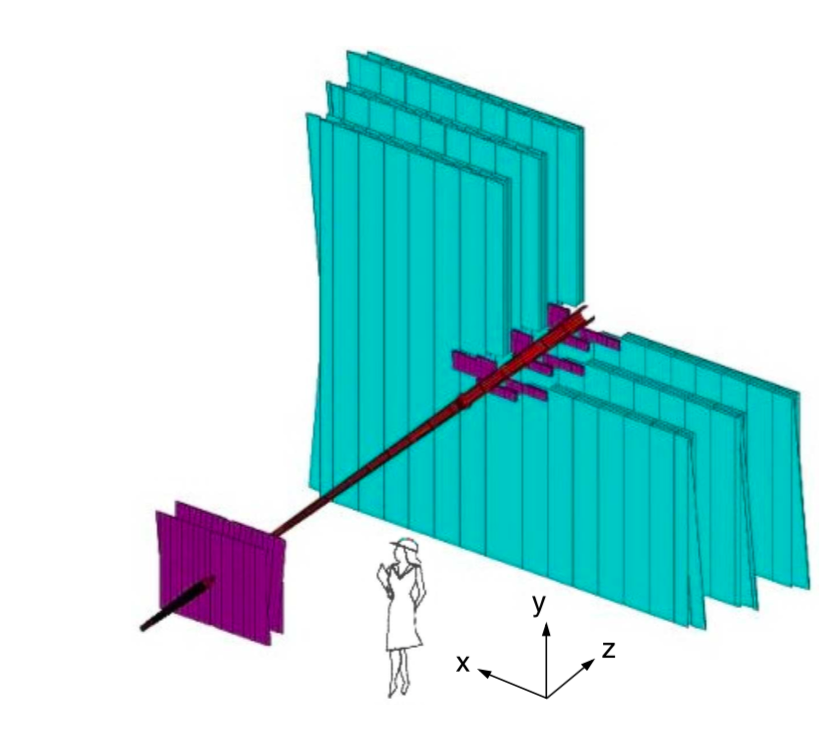
\includegraphics[ width=0.5\textwidth]{./Figs/LHC_LHCb/TT_IT_OT_comparison.png}
  \caption{TT, IT, OT comparison. Source: \cite{Alves:2008zz}.}
  \label{fig:types_of_tracks}
\end{figure}

The IT is very similar in design to the TT, it is make of 4 layers of silicon trackers in each station with a track resolution of 50 $\mu$m.
%and has an active area of 4.0m2. 
The silicon trackers are arranged in a cross shape around the beam pipe, as shown in Figure X, although the cover less than 2$\%$ of the tracking stations 20$\%$ of tracks pass through them. This allows the occupancy of the OT to be less than 10$\%$ so that it can be made of something other than silicon and still give good overall momentum resolution. The OT of each tracking station is made of 2 staggered layers of straw tubes, they cover the remaining area required for cover the LHCb full angular acceptance which includes tracks bend by the magnetic field of the magnet. The tubes have a fast drift time of 50 ns which enables a better than 200 $\mu$m track resolution. 


\subsubsection{The Dipole Magnet}
\label{Magnet}
A warm dipole magnet is used to measurement the momentum of charged particles travelling through the LHCb detector. In a magnetic field the trajectories of charged particles are bent and from the radius of curvature of the particle track the momentum of said particle can be determined.

The magnet is located between the TT and the tracking stations T1-3 and it’s field covers the full LHCb acceptance. The field is in the vertical direction therefore bending tracks in the horizontal direction. The magnet was designed so that it’s strength in the RICH detectors is negligible (less than 2 mT) and to have the largest strength possible between the TT and T1-3. Figure \ref{fig:Magnet_field} shows a plot of the magnet strength overlaid on the detector. A small magnetic field is achieved in the RICH detectors by shielding. The magnet was therefore designed to have an integrated field strength is 4Tm for track that travel 10m and the peak strength is 1.1T. % I should maybe mention the measurement of the field and how it had to be accurate (with Hall probes) in order to get good momentum resolution but I don’t want to.

\begin{figure}[htb]
  \centering
  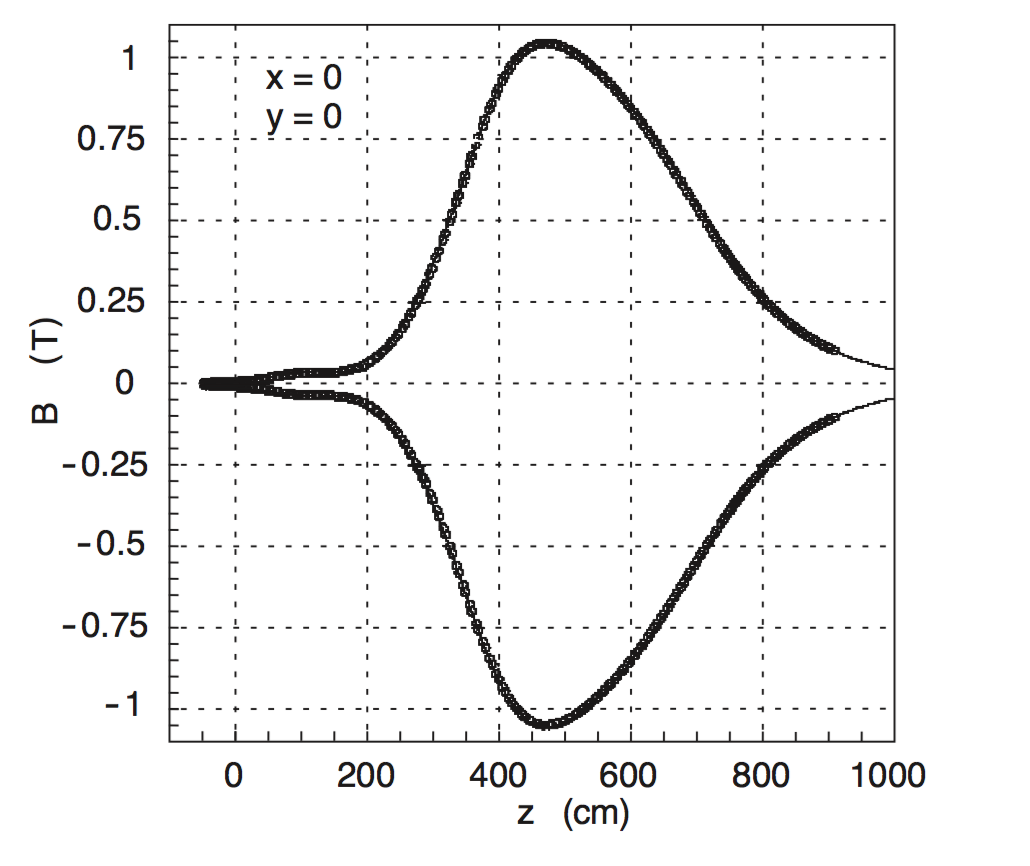
\includegraphics[ width=0.5\textwidth]{./Figs/LHC_LHCb/Magnet_field.png}
  \caption{Magnet field \cite{Alves:2008zz}.}
  \label{fig:Magnet_field}
\end{figure}

%\begin{figure}[tb] 
%  \centering    
%  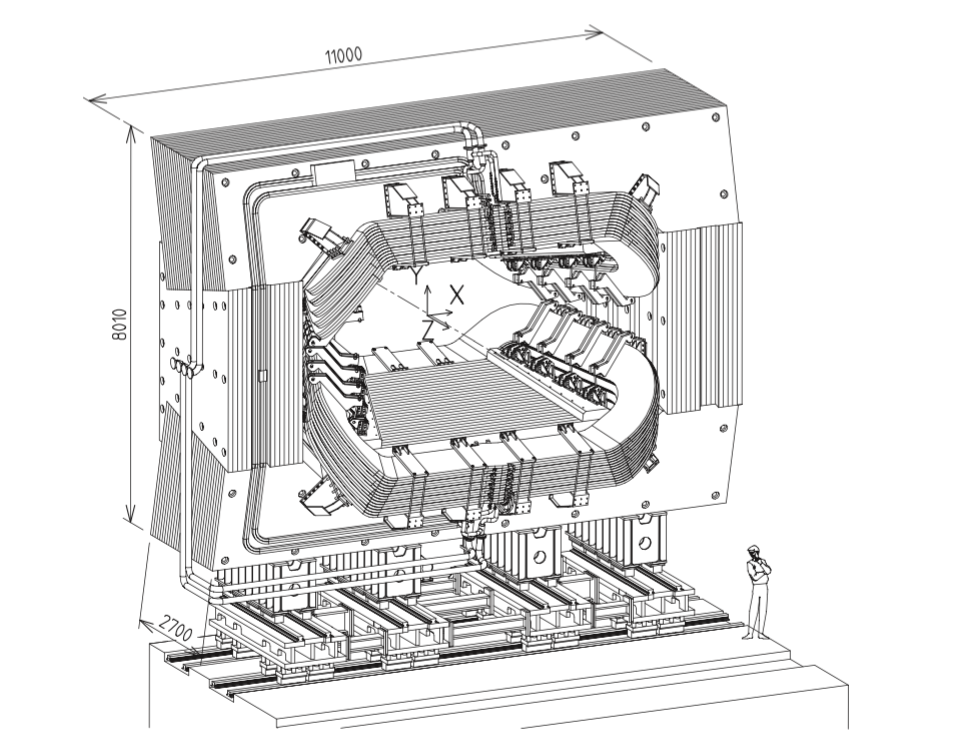
\includegraphics[ width=1.0\textwidth]{./Figs/LHC_LHCb/Magnet_picture.png}
%  \caption{Magnet picture. Source: \cite{Alves:2008zz}.}
%  \label{fig:types_of_tracks}
%\end{figure}


The polarity of the magnetic field is periodically switched therefore bending charged tracks in opposite directions. This is done so that left-right detection asymmetries can be measured and it helps with the systematic uncertainties of CP violation measurements. % These are not relevant for B2mm.



\subsubsection{Track resconstruction and Preformance of the tracking}
\label{Track_recon}


The information left by the passage of charged particles in each of the VELO, TT and T stations are combined using track reconstruction algorithms for determine the passage of charged particles through the detector. The algorithms start with either segments of tracks in the VELO or the T stations as seeds and then extrapolate using these segments into the other tracking detectors joining tracking in specific search windows in each detector. The rescontructed tracks are classified into five different types depending on what signature they left in each detector. The different types of tracks are illustrated in Figure \ref{fig:types_of_tracks}. 

\begin{figure}[htb] 
  \centering    
  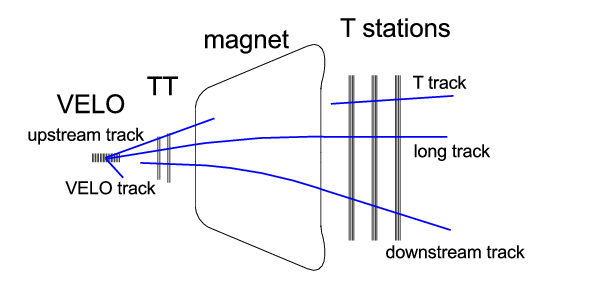
\includegraphics[ width=0.8\textwidth]{./Figs/LHC_LHCb/Types_of_tracks.png}
  \caption{Different types of tracks that are reconstructed at LHCb. Source: \cite{Aaij:2014pwa}.}
  \label{fig:types_of_tracks}
\end{figure}



VELO tracks come from particles that only leave information in the VELO, these tracks usually are at a large angle or are travelling backwards and are useful in reconstructing primary vertices.

Upstream tracks are formed by low momentum particles that are only observed in the VELO and the TT because they are them swept out of the detector acceptance by the magnetic field. These tracks have a poor momentum resolution but are useful for understanding backgrounds and pattern recognition in the RICH 1 which is located between the VELO and the TT provided the particles have sufficient momentum to be seen in the RICH.

Downstream tracks come from decay of the long lived particles, these particles do no leave information in the VELO only the TT and T stations. 

T tracks are tracks that only cross the T1-3 station and are formed from particles created from interactions with the material in the detector. Similarly to upstream tracks, T tracks can help to understand backgrounds and pattern recognition in the RICH2 which is located just before the T stations.

Long tracks are the most useful for physics analyses because they are formed from information left in the VELO, TT and T1-3 stations and consequently these tracks have the best momentum resolution.

The efficiency to correctly reconstruct tracks depends of different parameters of the events, such as the momentum to the particle producing the track, for long tracks they are correctly reconstructed on average of 96$\%$ of the time as shown in Figure XX for Run 1 data. 

Tracking efficiencies were measured using tag and probe method with Jpsi2MuMu, the average effieicny is better than 95 $\%$ for the mometum range 5 - 200 GeV and pseuoradify range 2-5 for Run 1. % (this is pretty much a quote from the paper. There are lots of plots in the paper so I think I should leabe them out!
Once the segments of the track have been found the trajectory is fitted with a Kalam fitter with takes into account multiple scattering and energy loss within the detector. For each track the fitter returns the chi2/ndof for each track which is a measure of quality for the track. In LHCb this parameter is used to ensure that only ‘good’ tracks are used in analyses. 

Inevitably every track that is reconstructed is not correct, there are two main types of incorrectly reconstructed tracks. The first is clone tracks that occur when the two tracks share many hits in common, when this happens the track with the highest number of total hits it used and the other is discarded. The second type of incorrect track are ghost tracks when segments in different detectors are incorrectly joined together, this can happen with tracks in the VELO and T1-3 stations, the number of times that this happened depends on the multiplicity of an event. These tracks are remove by cutting on the output of a neural network that returns a probability of how likely a track is to be fake.



Once the tracks have been reconstructed this allows the computation of different parameters that are necessary for the identifying different b hadron decays. The performance of the tracking system has been studied of Run 1 data \ref{ performance paperS}. The tracking system provide measurement of the momentum of the charged particles that it tracks, good momentum resolution is required in order to obtain good mass resolution which is necessary to identify different  b hadrons and to distinguish between signal and background events. The momentum resolution of long tracks is shown in figure  OR the momentum resolution is $\delta$p/p = X - Y $\%$ which depends on the momentum of the reconstructed track. 


The tracking system allows accurate reconstruction of primary verticies, this is necessary to measure time dependant processes, lifetimes and identify decaying particles. It was particular important for LHCb so that is could measure the rapidly oscillation Bs system. The PV resolution has been measured on 2012 data and varies with the number of tracks used to reconstruct the vertex, on average the vertex resolution transverse to the beam is between 10 and 25 mum and parallel to the beam is  between 50 and 150 mum for the z direction as shown in figure \ref{fig:types_of_tracks} for 2011 data. %Ref veto paper.



The impact parameter is another important variable, it measure the distance of closest approach of a track to the PV, long lived particles tend to have a large IP wrt to PV because they travel before they decay. Good measurements of the IP help to remove prompt backgrounds. The IP resolution depends on the momentum of the particles and Figure \ref{fig:types_of_tracks} shows the IP resolution for 2012 data, for a track with transverse momentum of 1 GeV/c is has an IP resolution of 35 mum.


Finally, the measurement of lifetime of b hadrons at LHCb needs accurate decay time measurements but more importantly to understand the rapidly oscillating Bs system good decay time resolution is needed. To reconstruct the decay time information about particle momentum and decay length, how far the particle travelled before it decays are needed. Therefore good PV resolution and moment resolution are needed. The LHCb detector achieved typically 50 ns resolution on the decay time. 

\begin{figure}[tb] 
  \centering    
  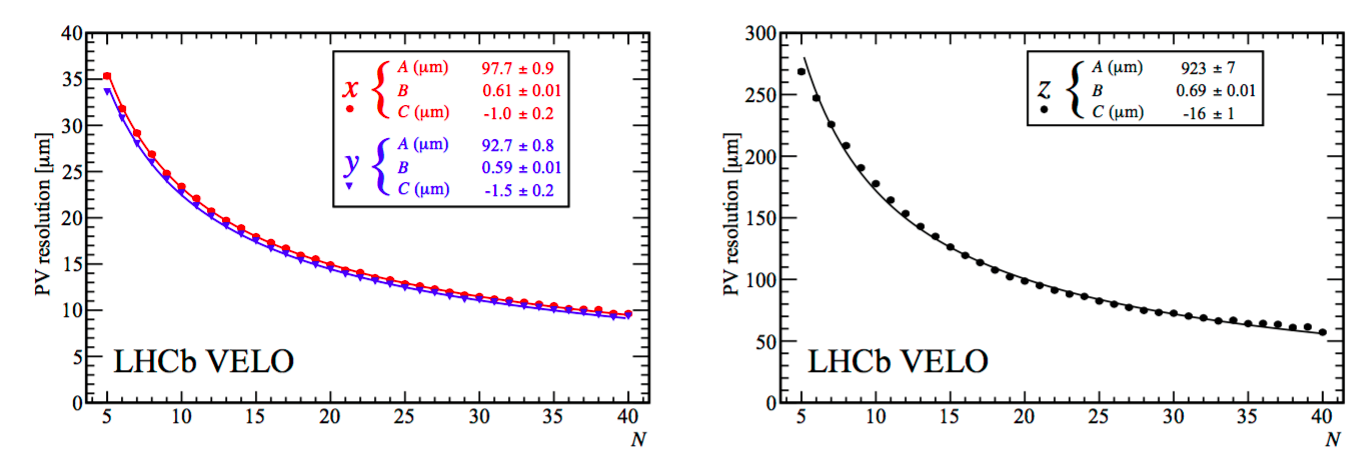
\includegraphics[ width=1.0\textwidth]{./Figs/LHC_LHCb/Velo_vertex_resolution.png}
  \caption{Velo prefomance. Source: \cite{LHCbVELOGroup:2014uea}.}
  \label{fig:types_of_tracks}
\end{figure}



\begin{figure}[tb] 
  \centering    
  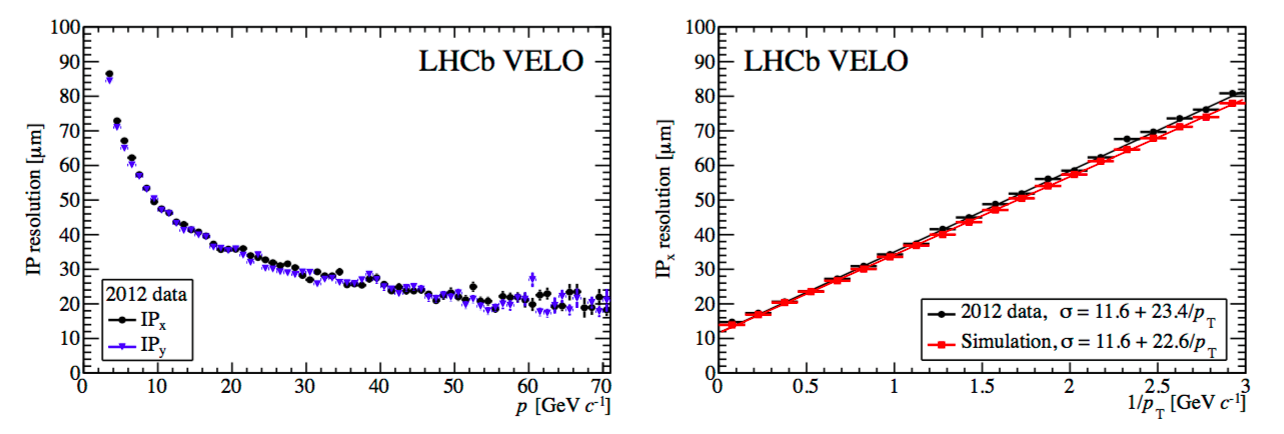
\includegraphics[ width=1.0\textwidth]{./Figs/LHC_LHCb/Velo_IP_resolution.png}
  \caption{Velo prefomance. Source: \cite{LHCbVELOGroup:2014uea}.}
  \label{fig:types_of_tracks}
\end{figure}




\begin{figure}[tb] 
  \centering    
  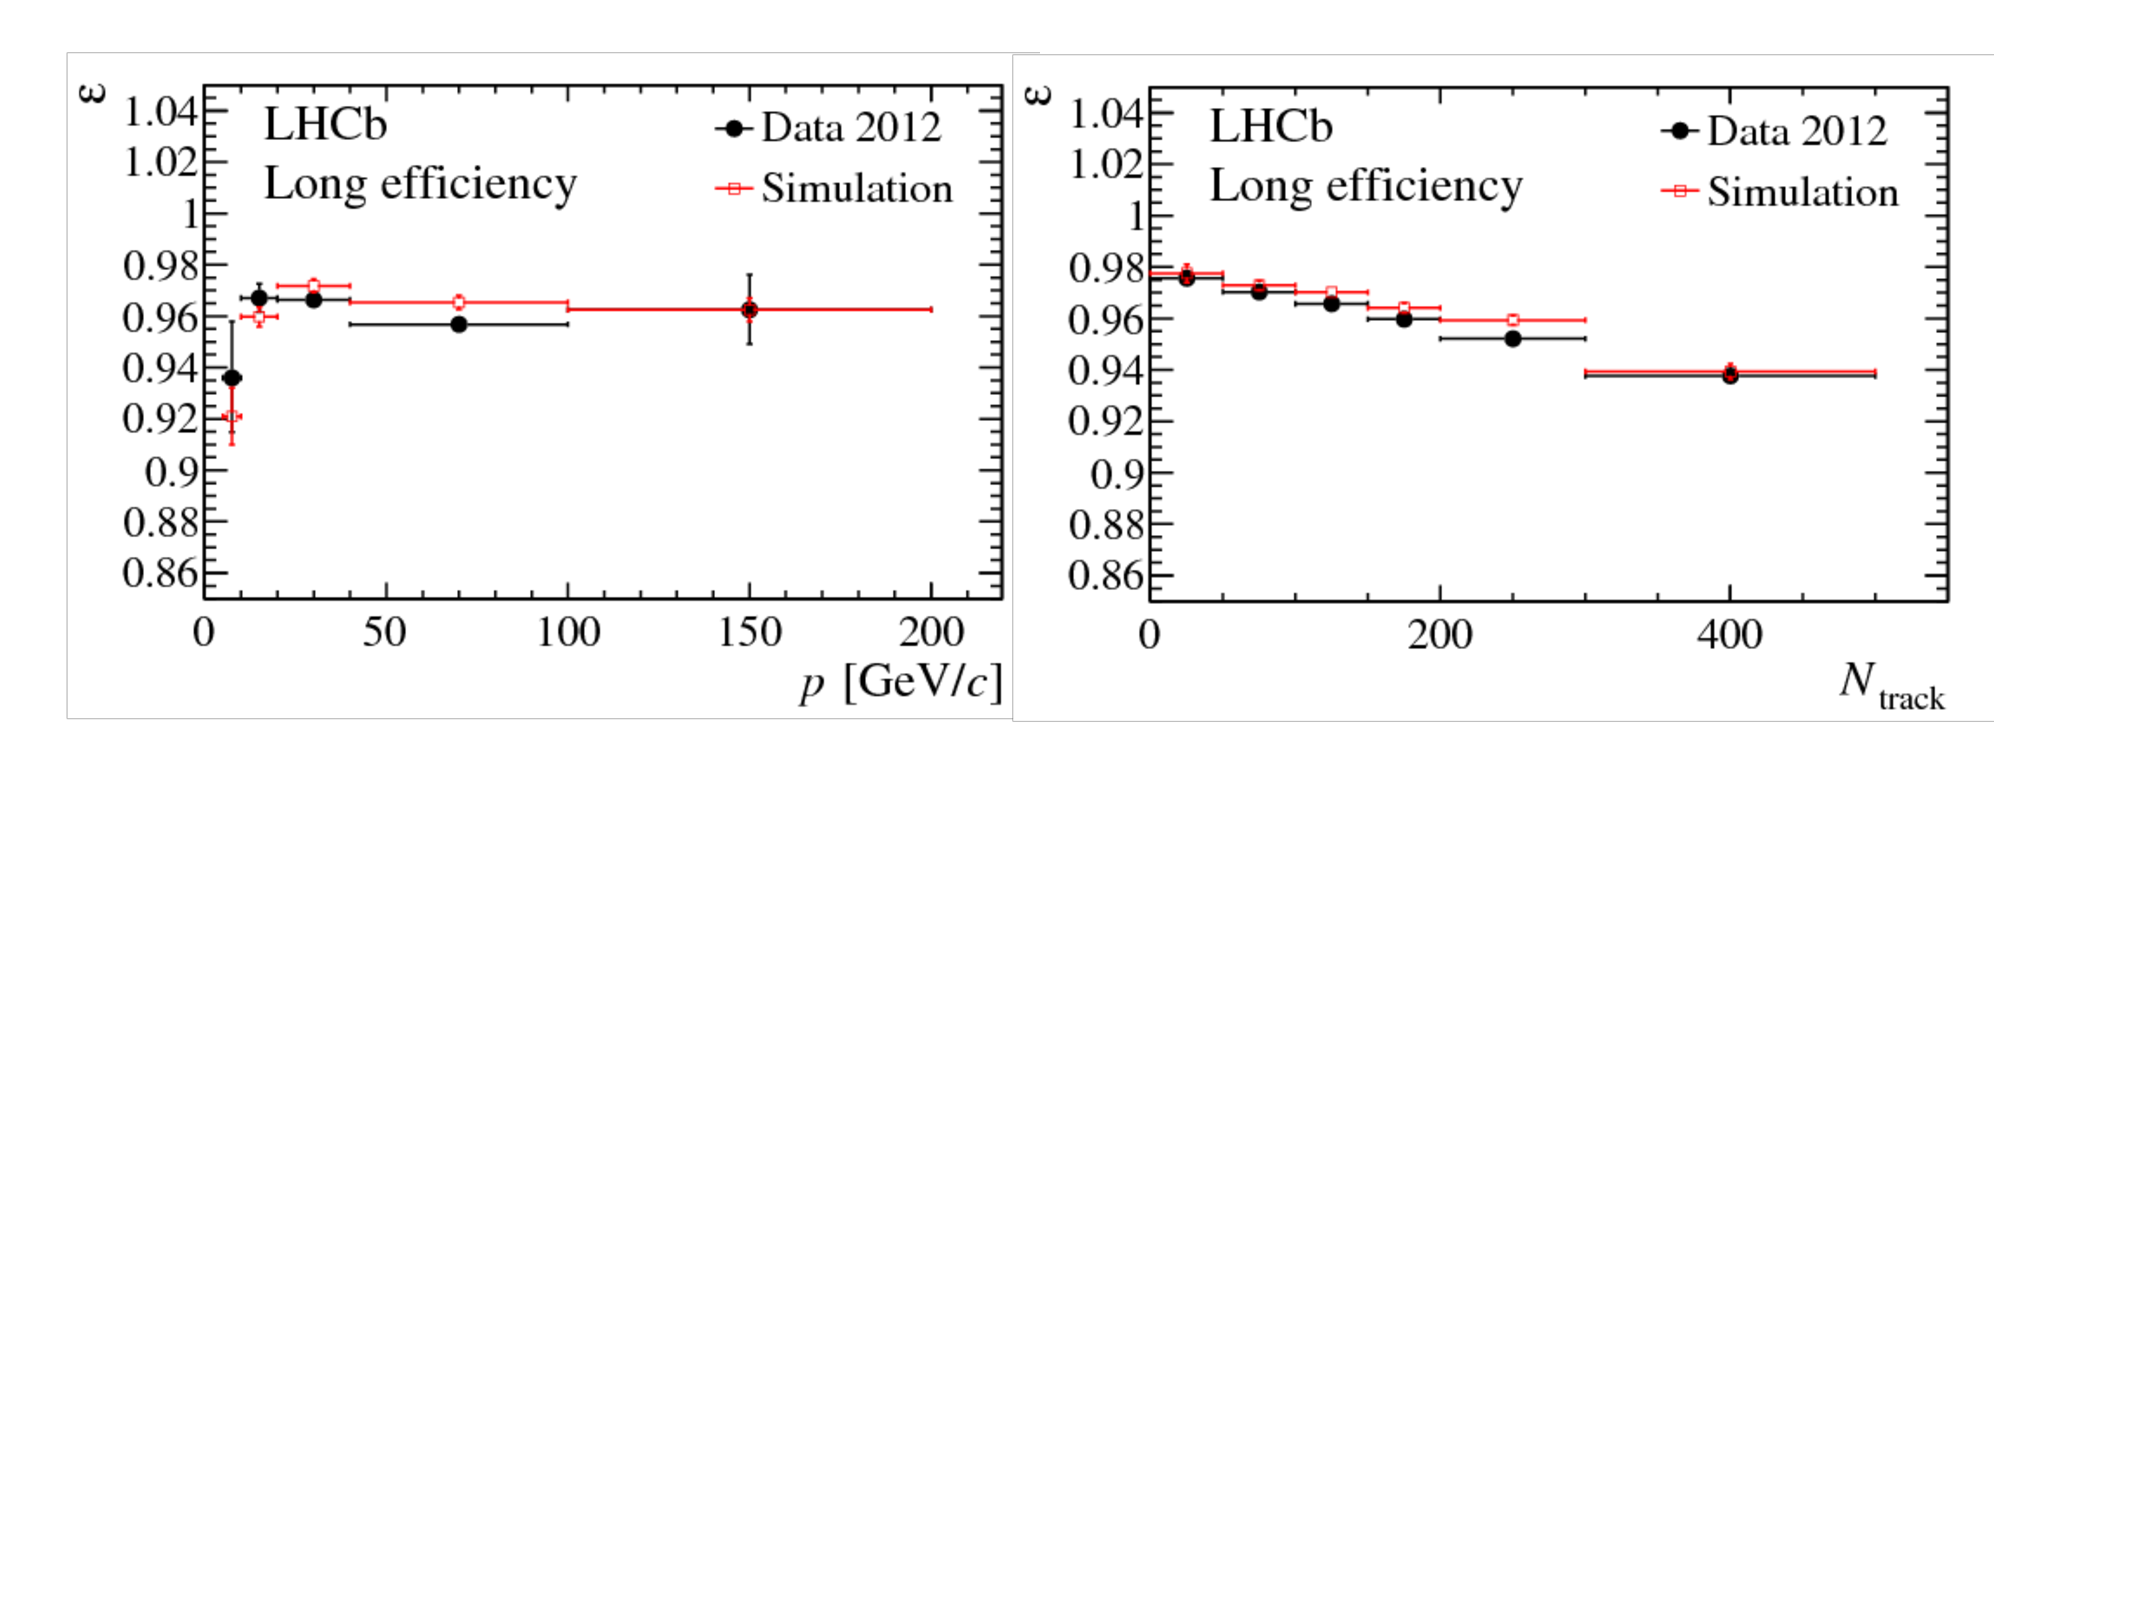
\includegraphics[trim = 1mm 150mm 1mm 1mm, width=1.0\textwidth]{./Figs/LHC_LHCb/LongTrack_efficiencies.pdf}
  \caption{Source: \cite{Aaij:2014pwa}. There is also 2010 and 2011, and other variables so prehaps put no image and just says it's around 96$\%$ for Run 1.}
  \label{fig:types_of_tracks}
\end{figure}










\subsection{Particle Identification}
\label{PID}

In LHCb the particles identification detectors consist of two ring imaging cerenkov detectors, an electromagnetic and hadrons calorimeter and the muons stations. Together these detectors distinguish between different charged leptons and hadrons and between neutral particle such as photons from neutral pions that are produced in \bhadron decays. Good particles identification is necessary because accurate identification of daughter particles identifies what b hadron decayed and also it is necessary to distinguish between topologically similar decays, such as b2pipi, b2pik, b2mumu. %This could be out elsewhere prehaps in the RICH specific part?
\subsubsection{RICH}
\label{RICH}
%There is a plot that shows the usefulness of the RICH PID, this is in Ed Greening's Thesis. 
RICH detectors are used at LHCb to distinguish between charged hadrons and leptons that have a momentum between X and Y GeV/c, the main goal for the RICH is to distingush between pions, kaons and protons. This needs to be done because correctly reconstruting the b hadron invarient mass relies on correctly identifying what it decayed into. Information from the RICH is particularly important at distingusihing different b2hh decays which is useful for this thesis. The energy range of the RICH detectors was chosen because the typical decay products of 2 body b hadron decays is around 50 GeV. The detectors are based on the following principle; when a charged particle travels through a dielectric medium excited atoms caused by the passage of the charged particle are polarized, if the particle is travelling faster than the speed of light in the medium then the excitation energy is released as a coherent wavefront. The angle the wavefront travels relative to the particle trajectory depends on the speed at which the particle was travelling in the following way;
cos_thetac = c/nv. 

There are two detectors that cover complimentary momentum regions. The RICH 1 detector is located between the VELO and the TT station, it covers the full LHCb angular acceptance and provides PID information on particles in the momentum range 1-60GeV/c. The RICH 1, is illustrated in Figure X, it contains two different radiator materials; at the front of the detector is a aerogel which is sensitive to particles with the momentum up to 10 GeV and behind the aerogel is a gas radiator which is sensitive to particles from 10 - 60 GeV. The aerogel radiation was removed after Run 1 of the LHC. As charged particles travel through the RICH 1 rings of light are produced. These are focused by spherical mirror on to Hybrid Photon Detectors, the radii of the detected rings provides information about how fast the particle was travelling. %The speed of the particles, when combined with information about it’s momentum from the tracking stations realise the particles mass and therefore it’s identity.

The RICH 2 detector is located upstream of the RICH 1, between the last tracking station and before the first muon station. The RICH 2 consists of a gas radiator sensitive to particles with a momentum range 50 - 100 GeV/c and the detection principle of the ring of light is the same as the RICH 1 as illustrated in figure X. Unlike the RICH 1 the RICH 2 detector does not cover the full LHCb angular acceptance but only +/- 120 mrad in the horizontal and +/- 100 mrad in the vertial direction where the higher momentum particles it is sensitive to are present, the other particles have been bent by the magnet out of this region. 
Both the RICH detectors usse HPDs, these are sheilded from the magnet field using iron sheets so that the field is of the order of 2mT on the HPDs, this allows accurate detection of light created within the RICH detectors. 
The rings of light collected by the RICH detectors when combined with information about it’s momentum from the tracking stations realise the particles mass and therefore it’s identity. Figure \ref{fig:RICH_preformance} shows how the cerenkov angle and momentum can be combined to identify different types of particles in the RICH 1 detector, there are distinct bands for each particle mass. Figure \ref{fig:RICH_radiator_predictions} shows what is expected for the different radiators.  



\begin{figure}[htb]
  \centering
  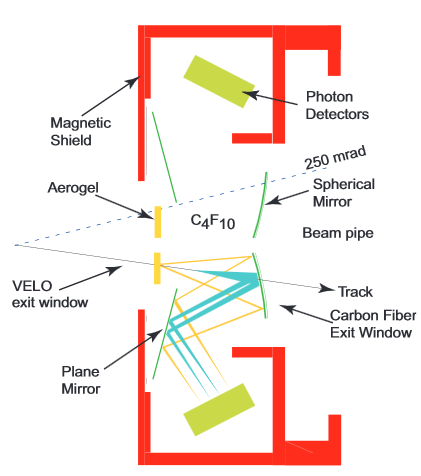
\includegraphics[ width=0.45\textwidth]{./Figs/LHC_LHCb/RICH1diagram.png}
  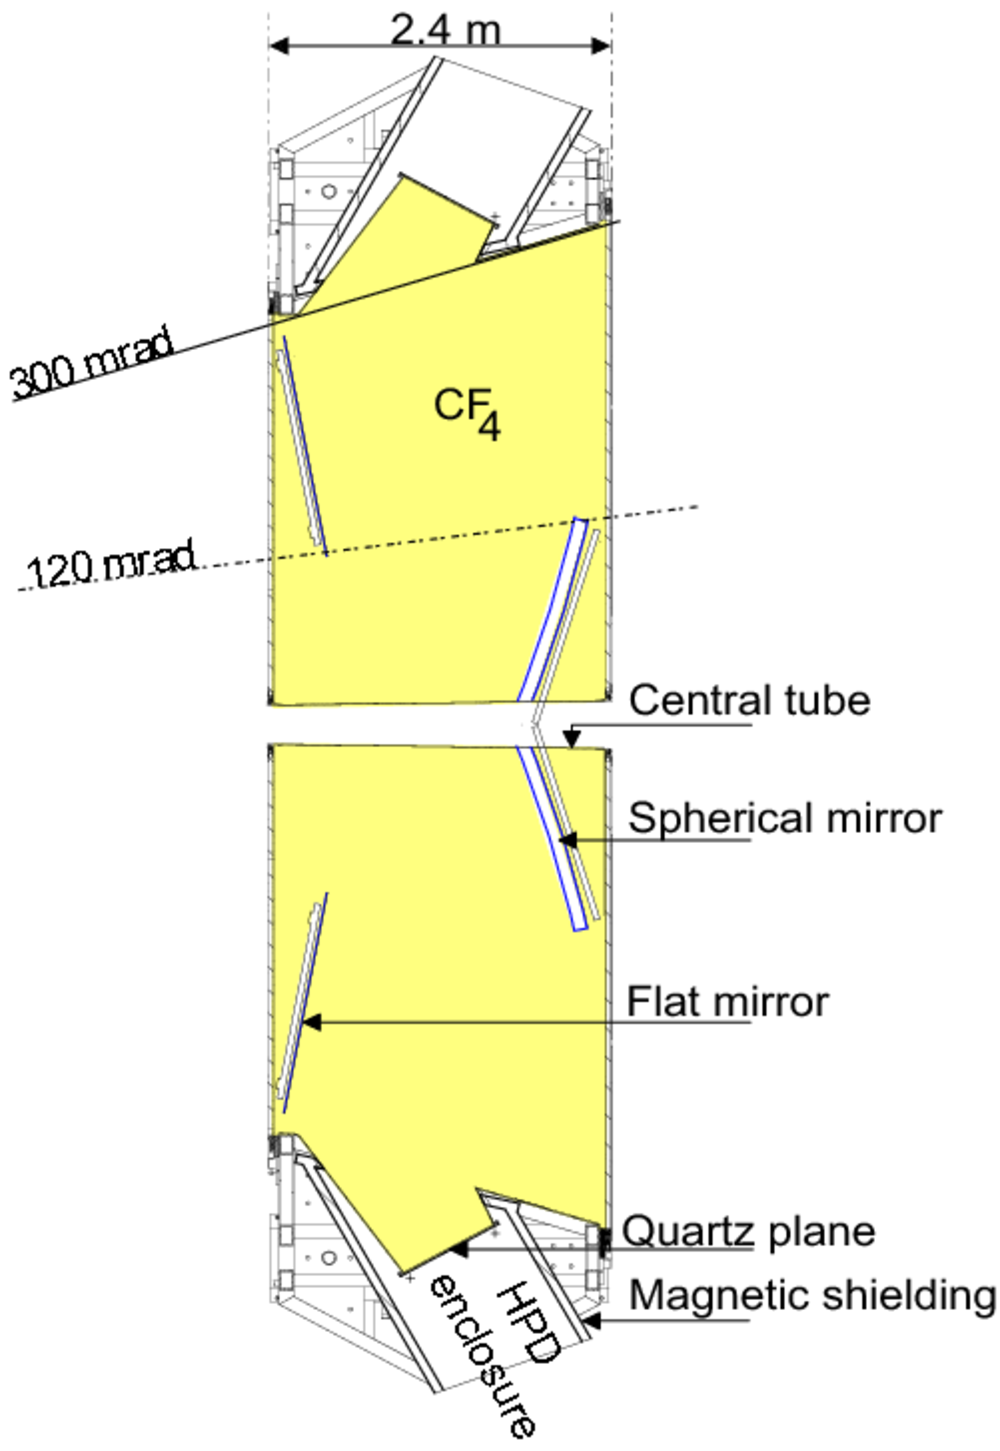
\includegraphics[ width=0.28\textwidth]{./Figs/LHC_LHCb/rich2_schematic.png}
  \caption{Diagram of the RICH1 detector \cite{Alves:2008zz}, also Olli has a nice picture of a HPD schematic.}
  \label{fig:RICH1_diagram}
\end{figure}


\begin{figure}[htb]
  \centering
  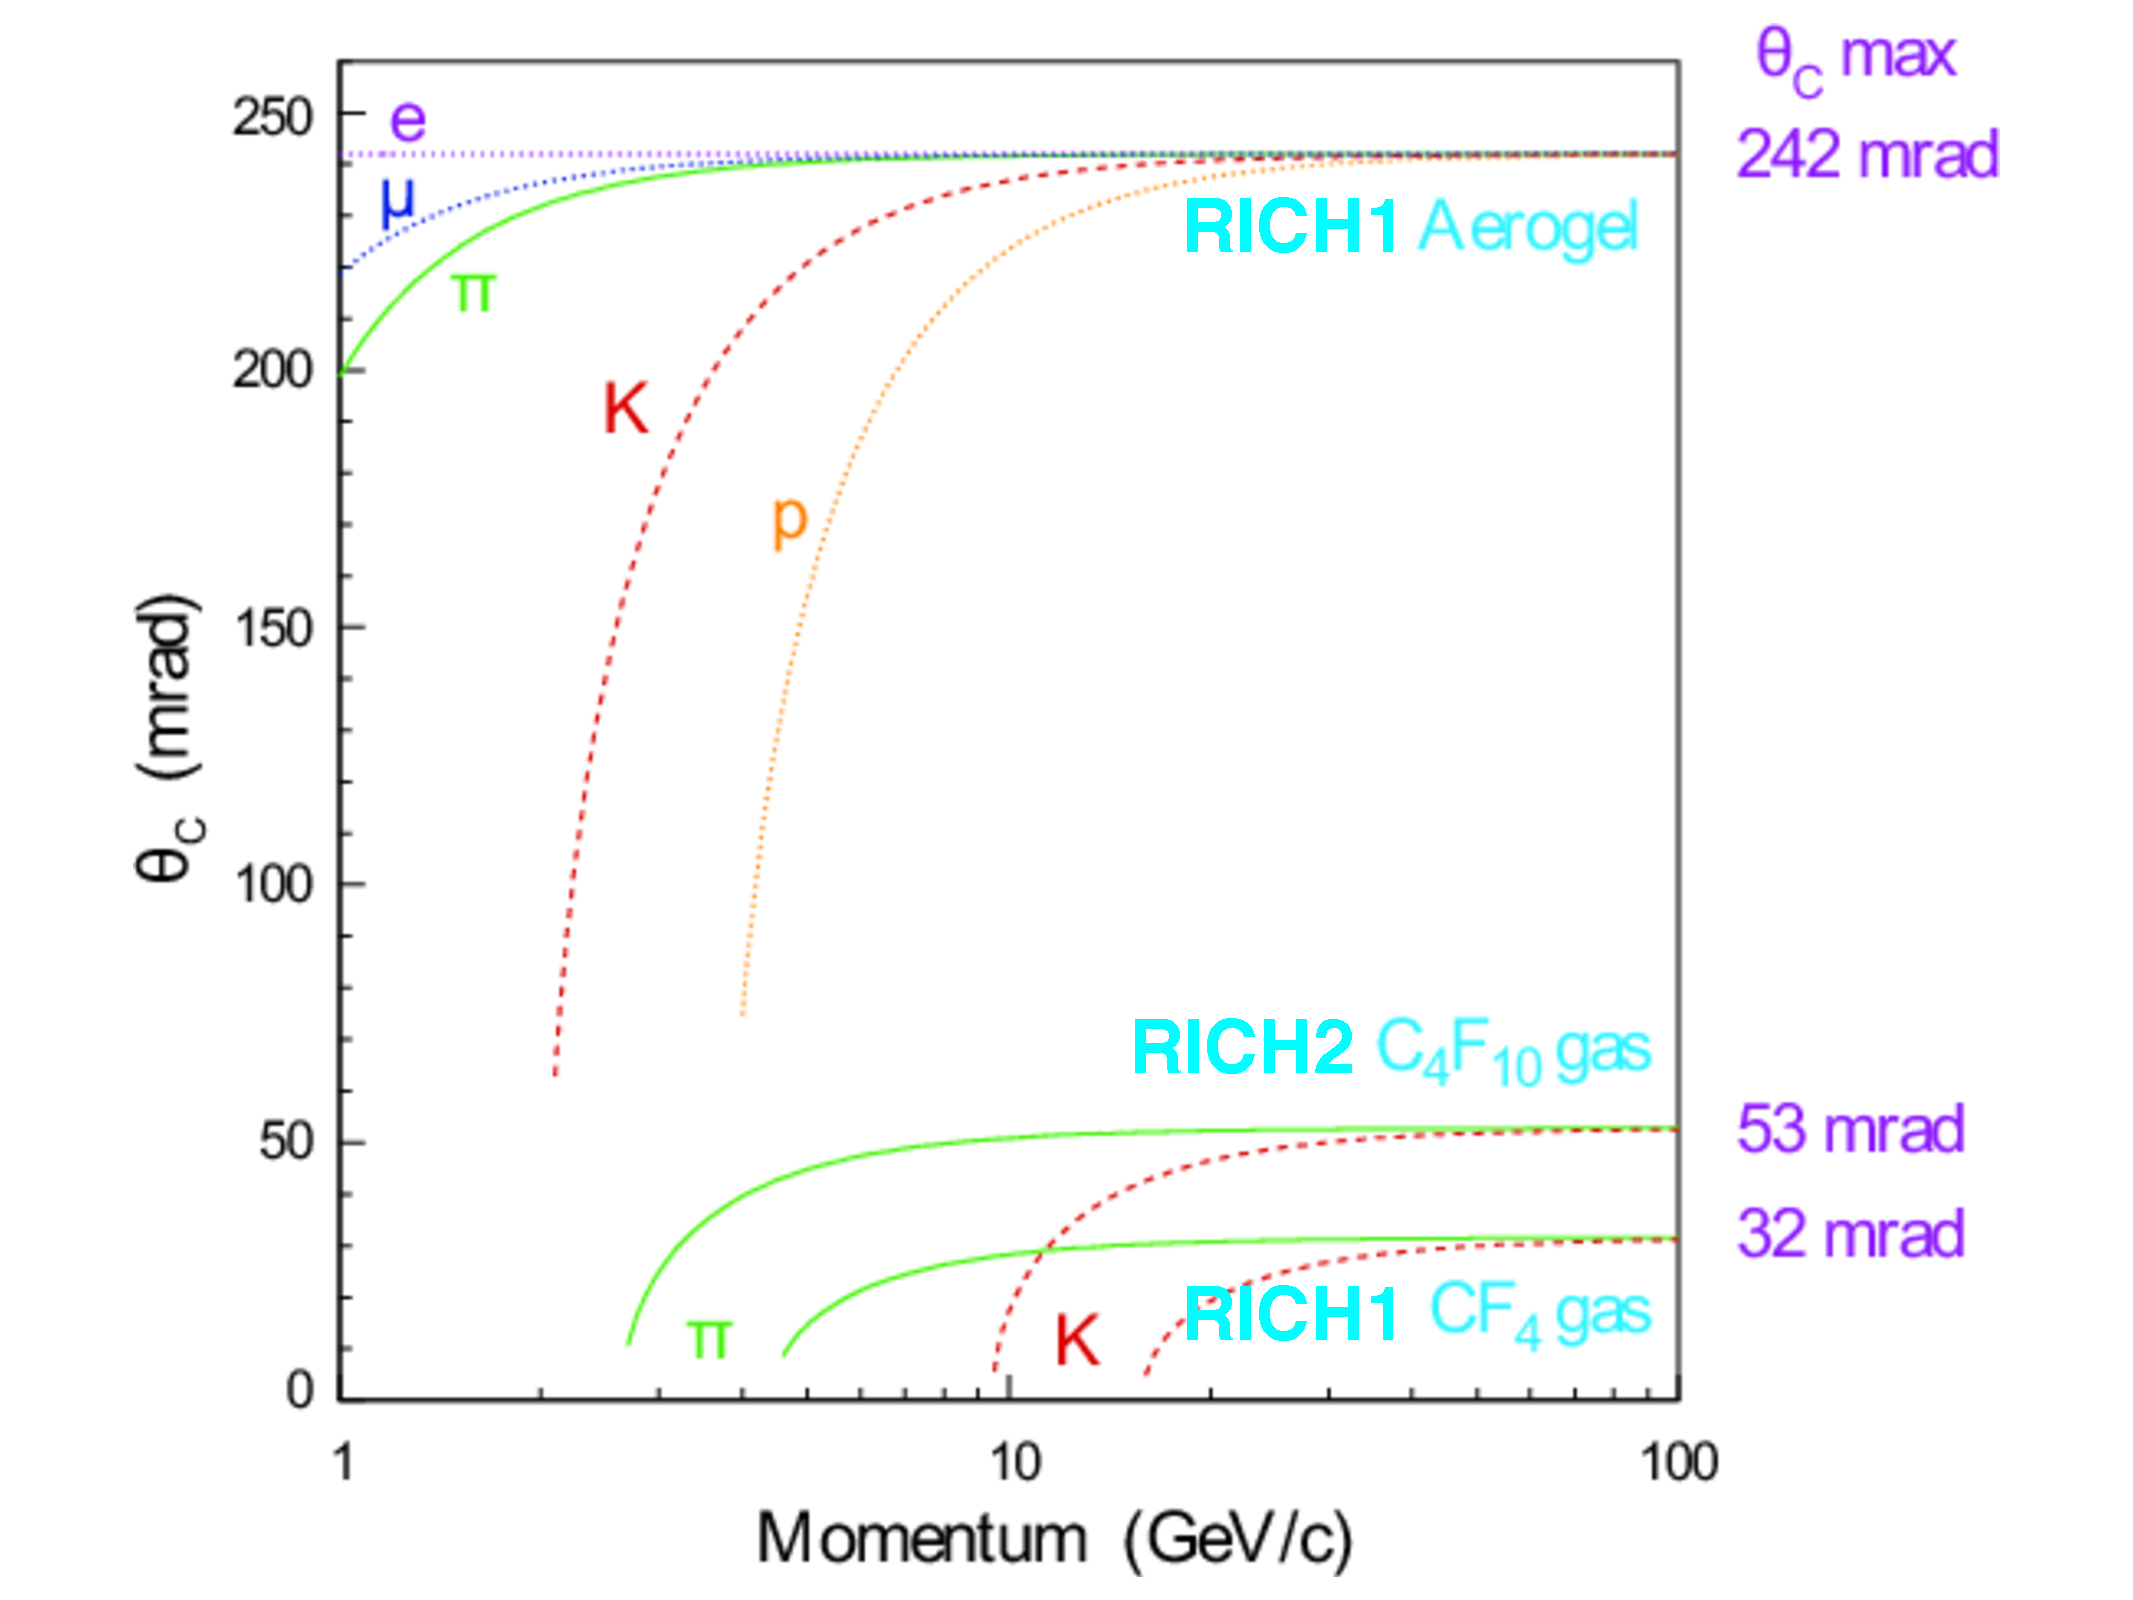
\includegraphics[ width=0.8\textwidth]{./Figs/LHC_LHCb/RICH_radiators.pdf}
  \caption{ \cite{Alves:2008zz}.}
  \label{fig:RICH_radiator_predictions}
\end{figure}


\begin{figure}[htb]
  \centering
  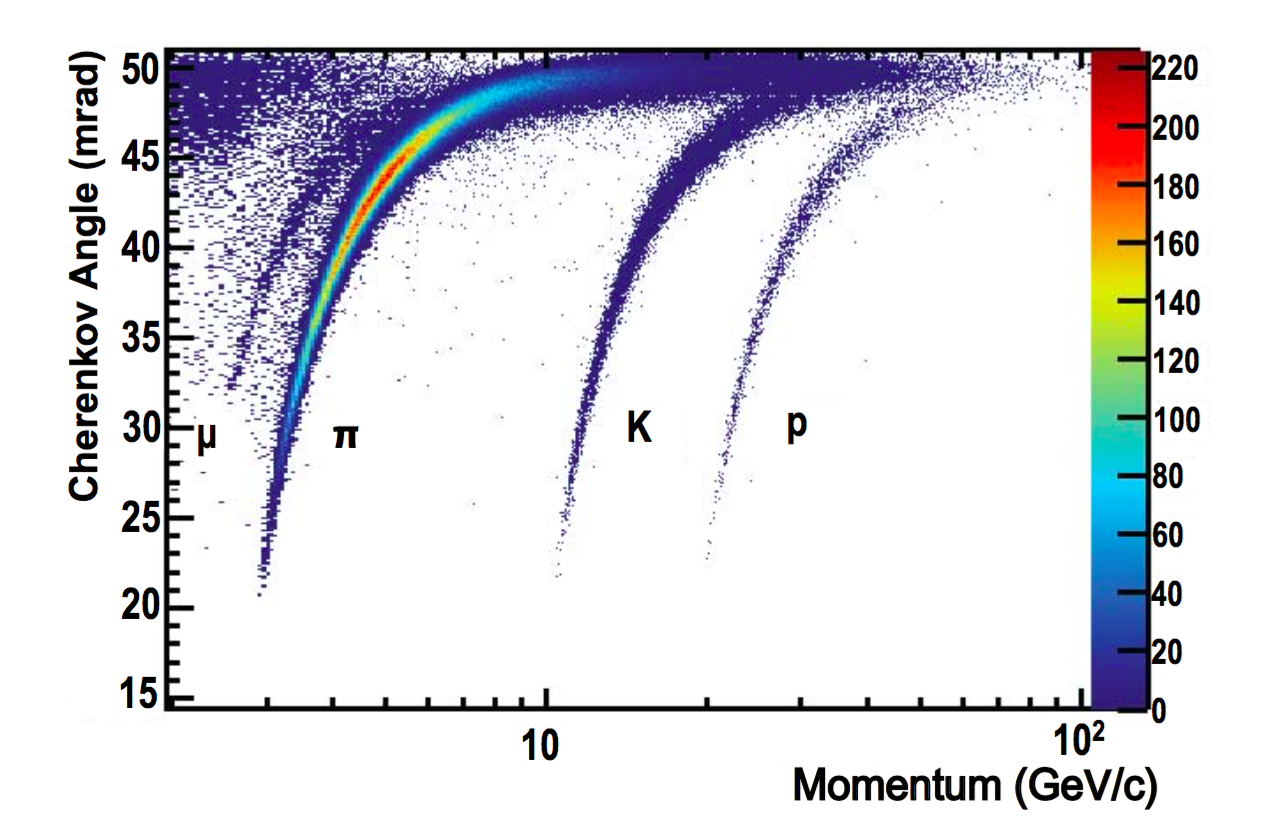
\includegraphics[ width=0.8\textwidth]{./Figs/LHC_LHCb/RICH1_performance.png}
  \caption{Performance of the RICH1 detector \cite{Adinolfi:2012qfa}.}
  \label{fig:RICH_preformance}
\end{figure}


\subsubsection{Calorimeters}
\label{Calo}

The calorimeter system in the LHCb experiment consists of the Scintillating Pad Detector (SDP), Pre Shower (PS), electromagnetic calorimeter (ECAL) and the hadronic calorimeter (HCAL). The main purposes of the calorimeters are to identify electrons, photons and hadrons with high transverse momentum to be used in the first level of the trigger the L0, and also to help with the reconstruction and identification of these particles. It is only the ECAL that will provide measurements on the position and energy of photons and neutral pions in the LHCb experiment. 

The calorimeters in LHCb are sampling calorimeters that consists of layers of lead and scintillating material. In the lead incident particles create showers of secondary particles which then produce light when the pass through the scintillators. This travels through a wave length shifter then is can be collected by photon multiplier tubes and turned into an electrical signal. In the ECAL showers are started by ionisation, bremstralung radiation or pair production depending on the energy of the incident particle and whether is it a $e^{\pm}$ or a photon. In the HCAL it is interaction via the strong force that leads to showers of secondary particles. 

The SDP, PS and ECAL all work together to identify electrons, positrons and photons. The SPD is a layer of scintillating material allows separation of election and photon showers created later in the calorimeter. This is because it is only charged particles that will produce light in the scintillator and the photons will not. The PS consists of a lead absorber followed by another scintillator similar to the SPD, the length of the lead absorber is chosen so that elections will start showers in the absorber but pions will not. There is only a 1$\%$ chance of a pion creating shower in the PS. Information collected by the PS enable showers created by pions in the ECAL to be separated from those created by electrons and positrons. The SPD is to separate electrons and charged pions. The ECAL is designed to contain the entire shower of high energy photons so that it can provide good energy resolutions of photons passing through the detector. The ECAL has an energy resolution of $\delta E / E = 9\%/\sqrt{(E)} \oplus 0.8\%$  provided information from the PD and SPD are used. 

The HCAL is predominately designed for use in the trigger and there is no requirement that the HCAL contains the full hadronic showers, therefore it was designed with an energy resolution of $\delta E / E = 69\% / \sqrt{(E)} \oplus 9\%$. 


\subsubsection{Muon Stations}
\label{Muon_stations}

\begin{figure}[htb]
  \centering
  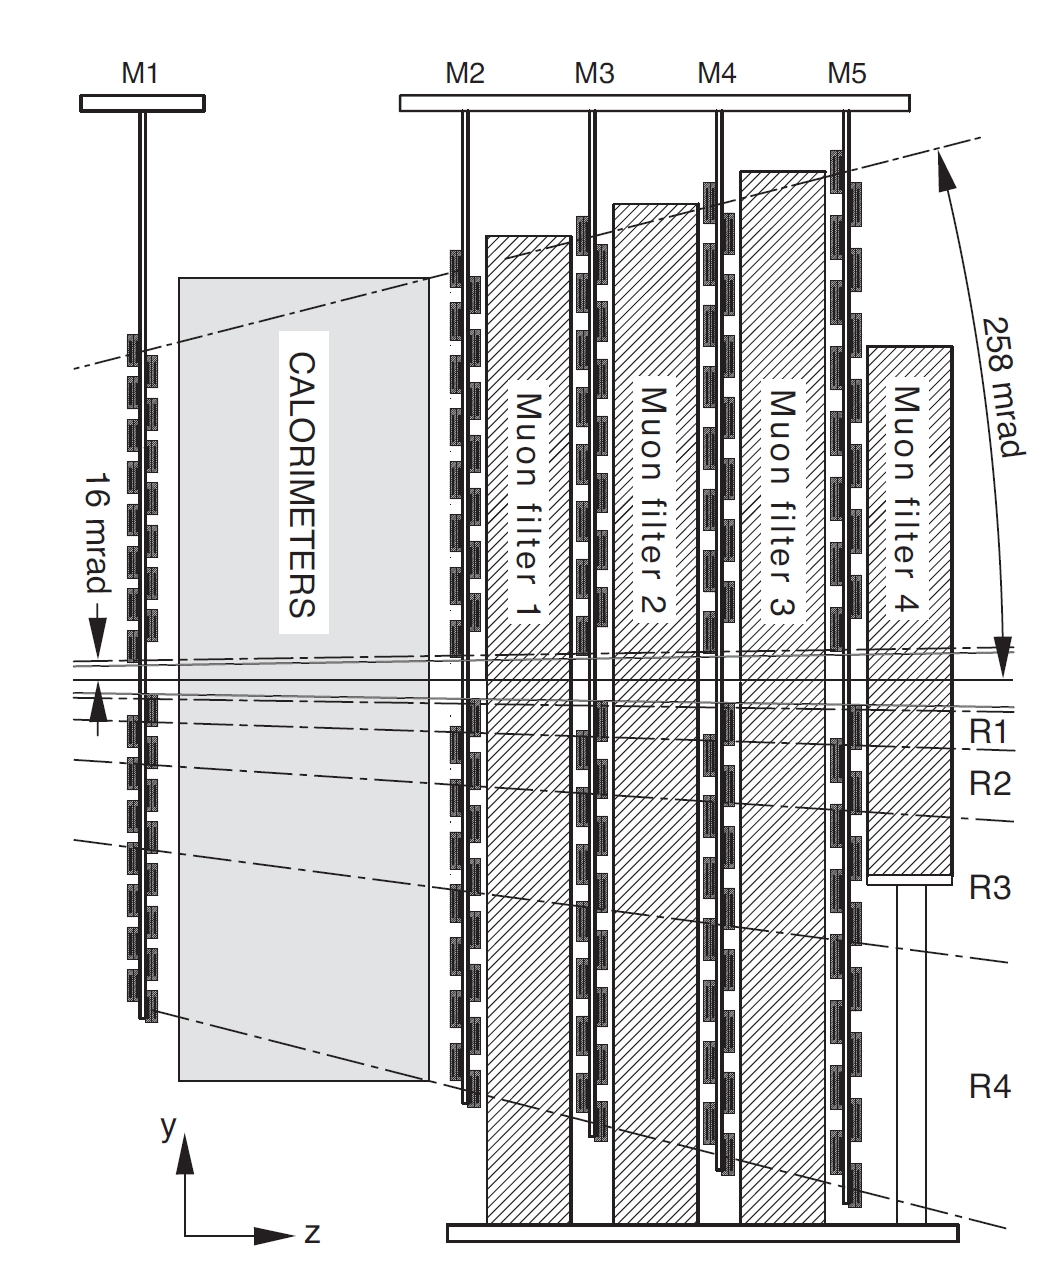
\includegraphics[ width=0.5\textwidth]{./Figs/LHC_LHCb/muon_system.png}
  \caption{Muon system \cite{Alves:2008zz}.}
  \label{fig:muon_system}
\end{figure}

The muons stations are desigend to identify highly penetrating muons, the information is used in the trigger and also in offline analyses. Muons are produced in from many \bhadron decays, some decays are topologically similar to \bhadron decays that do not include muons such as Bs2MuMu, Bd2KPi, Bs2KK, Bd2pipi. Therefore good muon identification is vital for triggering these events and enabling accurate reconstruction of events. 
Compared to other particles muons have a high penerating power due to their realtively large mass and because muons do not interact via the strong force, these proties are exploited in the muon detectors. 

There are 5 muon stations, M1-5, that work together to provide track and identigy highly penerating muons. The first muon station is located before the calorimeters, it's inner section is where the fluence is greater is make of gas electron multipler foils and it's outer section is made from MWPC. Stations M2-5 are located after the HCAL, by which point most other partciles have been absored by the calorimeters. These stations are made from MWPC and between each station is 80cm of lead absorber which ensure only highly penetrating muons pass through the muon detector. A muon must have a mometum of at least 3 GeV/c to pass through the calorimeters and M2 and M3, to travel through all the muons stations a muon must have a mometume of 6 GeV/c. 
The first 3 stations have a high spactial resolution and provide track and PT meinformation to be used the the trigger. M1 is located before the calorimeters to improve the PT measurement. The last two stations have lower spatial resolution and are designed to identify highly penetrating muons. After the muon stations there is am iron wall to stop any particles from travelling downstream of the detector. The size of the muon stations increases with distance from the interaction point to ensure tat the full angular accetpance of the detector is covered. Tracking information collected in the muon stations can be use in the trigger because the station lie outside the magnetic field which allows for fast reconstruction of the tracks and a muon is identified if information in the muon stations can be matched with hits in the tracking detectors. 

\subsubsection{PID information and performance}
\label{PID_variables}
%There is a plot that shows the usefulness of the RICH PID, this is in Ed Greening's Thesis. 

The information collected in the PID detectors is useful to provide several discriminting varaible that can be used to identify muons, protons, kaons, pions and electrons.

The muon stations are used, along with information from the tracking system, to procude a binary selection (isMuon) which is used to identidy muons. The tracking system is used to extrapolate a field of interest within the muon stations, a muon is identified if hits in the muon stations can be combined with those from the tracking system within the field of interest. The number of the hits required in the muon stations depend on the mometum of the muon, muons with mometum in the range 3<p<6 GeV must leave hits in M2-3, those in the  mometum range 6<p<10 muon leave hits in M2-3 and either M4 or M5 and finally muons with mometum above 10 GeV must be observed in all the muon stations. Figure~\ref{fig:isMuon_efficiency} shows the efficiencyt for the isMuon selection for selecting muons and also the mis-identification for hadrons to pass this selection. The mis-ID rate is higher at for lower mometum particles, which is expected given there are less hits in the muons detectors. The main contribution is the mis ID comes from the kaons and pions that decay in flight, the  muons from these decays are then detected in the muon stations.


\begin{figure}[htb] 
  \centering    
  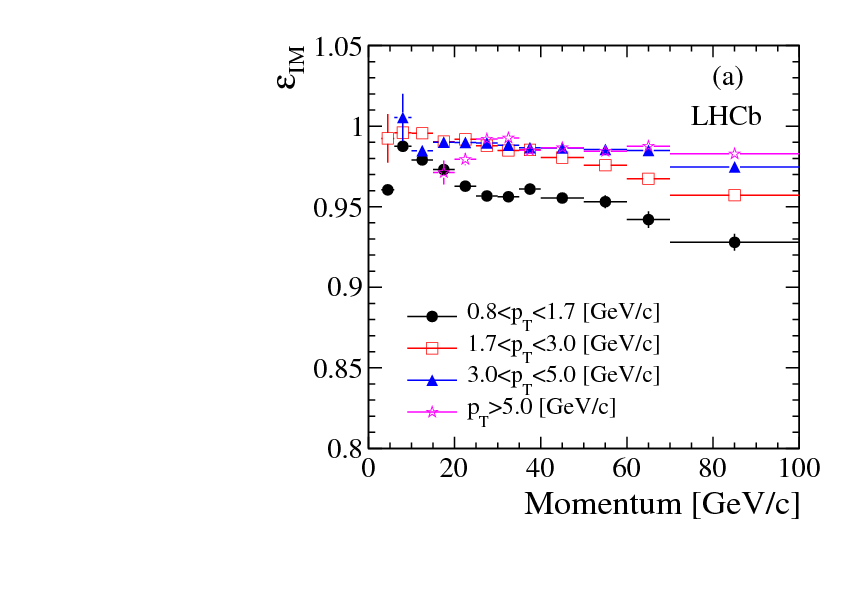
\includegraphics[ width=0.49\textwidth]{./Figs/LHC_LHCb/isMuon_signal_eff.png}
  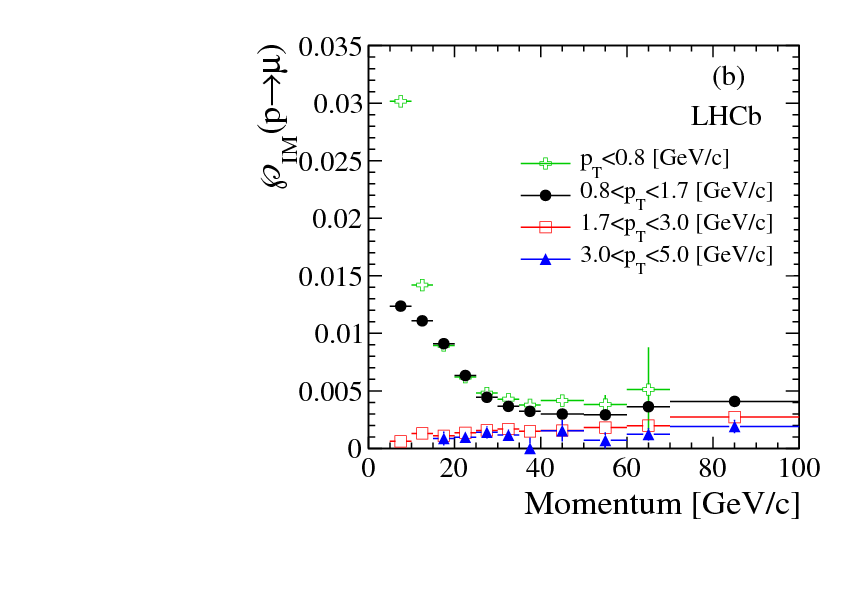
\includegraphics[ width=0.49\textwidth]{./Figs/LHC_LHCb/isMuon_rejection_eff_proton.png}
  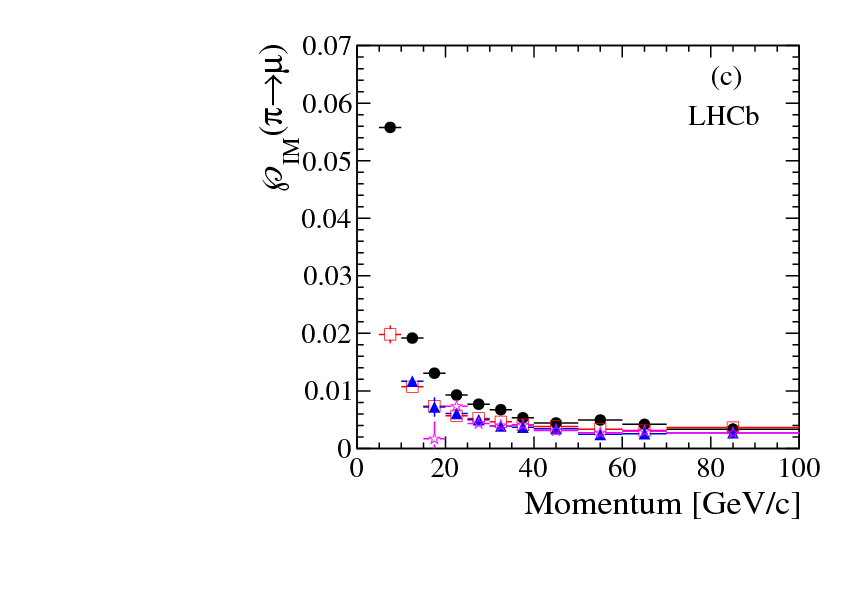
\includegraphics[ width=0.49\textwidth]{./Figs/LHC_LHCb/isMuon_rejection_eff_pion.png}
  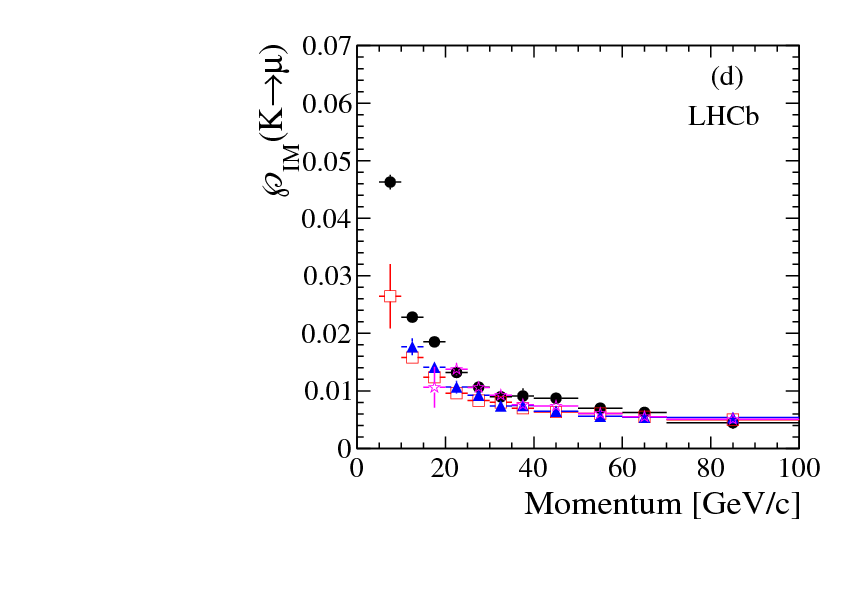
\includegraphics[ width=0.49\textwidth]{./Figs/LHC_LHCb/isMuon_rejection_eff_kaon.png}
  \caption{Place holder muon efficieny and misidentification probabilities \cite{Archilli:2013npa}.}
  \label{fig:isMuon_efficiency}
\end{figure}




The information from all the PID detectors is combined in two different way to provide global particle identification variables. One method is based on likelihood fits and the other is based on Neural Networks. In the first method, a likelihood fits are performed in each sub-detectorthat compare each charged particle track to different particle hypotheses. The information from the likelihoods in each sub detector is then combined into a global variable. This varible is the difference in the log - likelihoods between the track corresponding to a pion and a different particles hypothesis (kaon, proton, muon, electron), it gives a measure of how likely each particle hypothesis is compared to a pion. These variables are known as DLL variables. 




The second method uses information from the PID detectors and the tracking system in Neural Networks to provide a probability of a track having a particular partice hypothesis. This method takes into account correlations between detector systems and extract detector information that are not considered in the likelihood method. The Neural Networks are trained on simulated inclusive b decays and can be tuned to suit different situations such as the data taking year. The variables produced by the Neural Networks are known as ProbNN variables. 


Figure~\ref{fig:DLL_vs_ProbNN} shows a comparison of the preformance of the DLL and ProbNN variables for signal effeciency can background rejection in selection protons and muons. Although the performance to the two types of variables are quite different, the efficiencies of the variables vary with different kinematic properties of the decay, such as the momentum, and the properties of the variables measure are different Therefore the most approproate PID variable type to use depends on the situation it is being used in. 




\begin{figure}[htb] 
  \centering    
  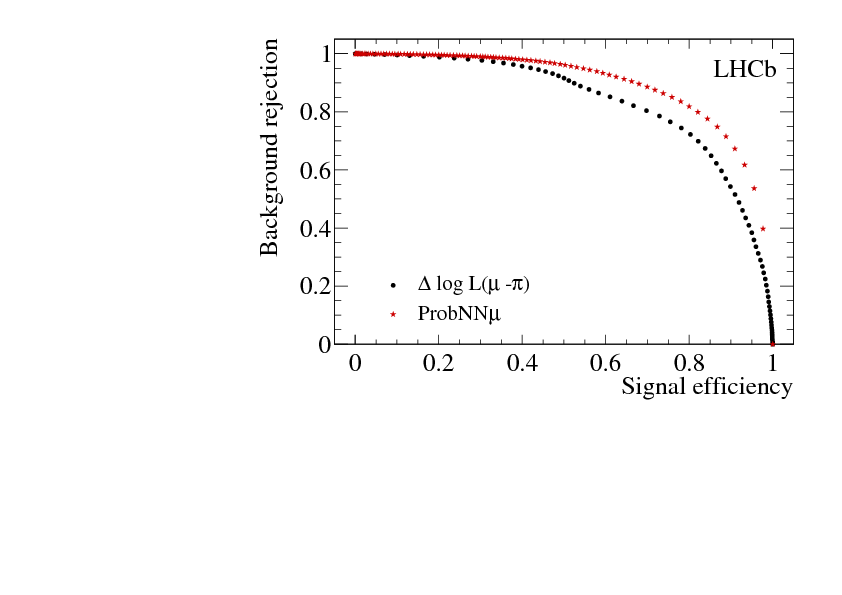
\includegraphics[ width=0.49\textwidth]{./Figs/LHC_LHCb/DLL_vs_ProbNN_muon.png}
  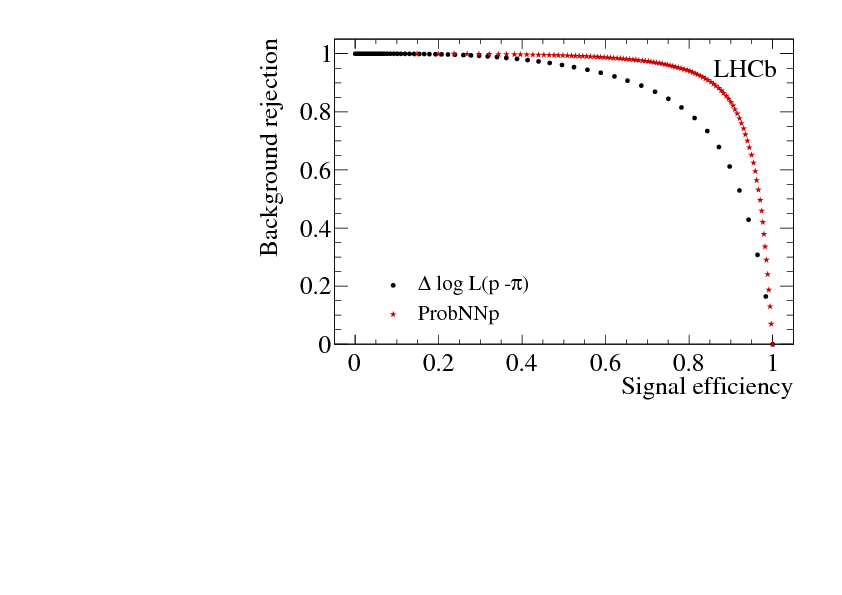
\includegraphics[ width=0.49\textwidth]{./Figs/LHC_LHCb/DLL_vs_ProbNN_proton.png}
  \caption{Muon and proton efficiency comparisons for DLL and ProbNN \cite{Alves:2008zz}.}
  \label{fig:DLL_vs_ProbNN}
\end{figure}







\subsection{The Trigger}

\label{Trigger}

The LHC was designed to collide protons at a rate of 40 MHz, this rate is too high for infomation to be read out of the LHCb detector. However most $pp$ collisions do not produce particles within the detector acceptance that are interesting for physics analyses at LHCb. A trigger system is used that selects potentially interesting events to be saved for later physics analysis. The trigger has been designed to select interesting physics events with a high efficiency  whilst reducing the event rate to one where information from the full detector can be read out.  There are two levels to the LHCb trigger; the hardware trigger and the software trigger. The hardware trigger is know as the level-zero (L0) trigger and reduces the 40 MHz event rate to 1MHz which is the rate at which the full detector can be read out. The hardware trigger is know as the High-Level-Trigger (HLT), it has two stages and runs on the output of the L0 further reducing the event rate by ultilising information for all the detector sub-systems. Each level of the trigger is composed of trigger 'lines'; these lines are made up of reconstruction and selection algorithms and either accept or reject each event. Only events that are acceptance by a trigger line at both the L0 and HLT analyses are avalible for physics analyses. 

\subsubsection{The L0 trigger}
\label{L0}


The L0 trigger runs synchronously to the LHC bunch crossing. Its purpose is to reduce the events rate to 1 MHz, where information from the full detector can be read out. Therefore the L0 is limited to use information from the detector that can be read at the same rate as the LHC collision rate.
The L0 uses information from 3 parts of the detector to make decisions about the relevance of each event; the VELO, calorimeters and the muon stations. 


The pileup veto stations in the VELO are used in L0 pileup trigger lines, these are relevant only for luminoscity measurements and will not be discussed further here.

The other L0 trigger lines are based on the kinematic propertices of \bhadron decays. The heavy masses of \bhadrons means that their decays are charaterised by the production of daughter particles with large transverse mometum ($p_{T}$) and transerse energy ($E_{T}$).
%The calorimeters are used to identify events that conatin electron, photons and hadrons with high $E_{T}$. 
The calorimeters are used to in trigger lines that select events containing high $E_{T}$ electrons, photons or hadrons. Information from the PS, SPD, ECAL and HCAL is used to identify electrons, photons and hadrons in each event. Events are then accepted by the trigger lines if there is an  electron, photon or hadron with $E_{T}$ above a threshold value provided the event multiplicty is not too high. The $E_{T}$ thresholds are different for each particle type. Events with high multiplicity take a long time to reconstruct and process in the HLT, therefore it is not efficiency to keep these events. The multiplity is measured by the number of hits in the SPD detector (nSPD), only events with nSPD lower than a specified value can pass an L0 trigger line. 


In a similar way to the calorimeters, the muon stations are used to identify muons with high $p_{T}$ for trigger lines. There are two L0 trigger lines for muons that accept events based on muon $p_{T}$ if either a single muon has a $p_{T}$  above a threshold value or if the two muons with this highest $p_{T}$ have $\sqrt{p_{T1} \times p_{T2}}$ above a threshold value, provided the event multiplicty is not too high. %The L0 muon trigger lines are most important to select \bsmumu candidates. The efficiencies for these 2 lines are show in Figure X, most eventa are triggered by the L0Muon but some are added by the L0Dimuon lines. 

The  $E_{T}$ and $p_{T}$ thresholds and the multiplcity limit for the L0 trigger lines vary for each year of data taking depend on the bandwidth avaliable for the trigger. % and are shown in table X. 


\subsubsection{The HLT trigger}
\label{HLT}

Events that are accepted by trigger lines in the L0 are moved to the Event Filter Farm where the HLT is run. The HLT is a software trigger that is split into two levels that are run sucessively. 


The HLT1 is the first level of the HLT. It runs on the output of the L0 checking the decisions make by the L0 trigger and reducing the event rate. % from 1 MHz for processing in the HLT2. 
Time constraints in the HLT1 do not allow for full event reconstruction using all LHCb sub-detectors, instead the HLT1 runs reconstruction and selection algorithms on even information from the VELO and tracking stations. These trigger lines are composed of generic selection criteria, making decisions that confirm those made in the L0 about particular particle types and also identify generic types of particle decay such as inclusive \bhadron decays. The second level of the HLT, HLT2, runs on the output of the HLT1 which provides an event rate that is low enough to allow event reconstruction that includes all detector subsystems. The trigger lines in the HLT2 are designed to select decays relevant to specific physics analyses or particle decay topologies, this is made possible by detailed information from the reconstruction. 

Just like the L0 trigger, trigger lines in the HLT vary for each year of data taking both the selection critera used in the lines and also new trigger lines are introduced. The number of HLT2 lines increases with each year of data taking as understanding of the capabilities of the experiment increases; there were about 100 HTL2 lines in 2011, 200 in 2012 and 450 in 2015. Furthermore, significant changes were made in the reconstruction used in the HLT between Run 1 and Run 2,  the details of the changes made can be found in CITE. The majority of the changes to the HLT for Run 2 are not relevant for the analysis discussed in this thesis, the overall impact is that a more detailed reconstruction is used in the decisions of the Run 2 HLT lines compared to Run 1.



\subsection{LHCb Software and Simulation}
\label{Software_Simulation}
%Options instead of referenes, Susan references the realease areas!

The data that is read out of the LHCb experiment needs further processing before it can be used in physics analyses. The \textsc{Gaudi} framework~\cite{Mato:1998gfa} is a C++ framework that is the basis for the software applications needed to process the data at LHCb~\cite{Antunes-Nobrega:835156}. This framework ensures that the necessary softeware is avaliable to all users and changes to the software are implmented accross all applications, it is suited to the distributed computing system used in LHCb~\cite{Stagni:2012rs}. 


Once events have been accepted by the trigger, the first step in processing the output of the detector is reconstructing events, this is done by the \textsc{Brunel} application. It takes the digitised detector read out and reconstructs hits in the tracking stations to find particle trajectories and momenta and combines information from the RICH detectors, calorimeters and Muon Stations to compute PID variables. The output of processing by the \textsc{Brunel} application are stored in `Data Summary Type' (DST) files. 

Next the \textsc{DaVinci} application is used to fit the tracks reconstructed in \textsc{Brunel} with primary and secondary verticies. This application at assigns particle hypotheses to each track and reconstructs the decay trees of particles in the detector, computing the kinimatic properties that are needed for physics analyses. The the reconstructed output of the trigger is too large to be stored in one place and to be used by all the analysts therefore a `stripping' proceedure is used to break up the data into a managable size for physics analyses. Each physics analysis designs a set of loose selection requirements specific to their decay of interest, the selections are applied to the reconstructed events and are designed to keep as much of the signal as possible but reduce the number background events. The output of this process are smaller DST files, events passing the stripping selections can either be saved with the full event information or with just the tracks related to the signal candidate. The choice depends on the physics process the stripping line is relevant for. The DaVinci application is then used one last time to produce \textsc{Root}~\cite{Brun:1997pa} files from the output of the stripping lines, these files display the data in histogram and are used for physics analyses. %RooFit has citation \cite{Verkerke:2003ir}


As well as data collected by the experiment, simulated data that mirrors what is expected in the experiment is needed to understand the detector performance and for physics analyses. There is a set of software applications that are dedicated to the production of Monte Carlo simulated events within the \textsc{Gaudi} framework. Events are generated using the \textsc{Gauss} application~\cite{1742-6596-331-3-032047, Clemencic:2011zza}, this package uses \textsc{Pythia}~\cite{Sjostrand:2006za,Sjostrand:2007gs} to model proton-proton collisions and the production of particles, then the \textsc{Evt}\textsc{Gen}~\cite{Lange:2001uf} application to calculate the decay of these particles. Final state radiation is modelled using \textsc{Photos}~\cite{Golonka:2005pn}. Both \textsc{Pythia} and \textsc{Evt}\textsc{Gen} have been tuned for the production and decay of particles within the LHCb detector. In the simulation the type of particles generated and how they decay can be specified so that the simulated events are relevant to particular physics decays. The detector response to the simulated events is processed by the \textsc{Boole} application with uses \textsc{Geant4}~\cite{Agostinelli:2002hh,Allison:2006ve} to model the detector. The output is a digitised reponse of the detector which is then processed by \textsc{Brunel} and \textsc{DaVinci} in the same way as the real data to produce \textsc{Root} files that are used in physics analyses. %RooFit has citation \cite{Verkerke:2003ir}

The LHCb software framework is set up so that it can be used on the Worldwide LHC Computing Grid~\cite{Bird:2011zz, WWCG}, the Grid is made up of computers across the world that each store part for the LHCb data set and simulation data. Despite the stripping process the data produced at LHCb is too large to be stored in one place. The \textsc{Dirac}~\cite{Paterson:1397926} system mananges grid site and use the \textsc{Ganga} project allows the submission analysis code to differnt sites. The grid enables analysts to be able to process and study the large amounts of data produced by LHCb without having to store the data where the analyst is. 





\subsection{LHCb data collected so far}
\label{LHCb_data}
%Need to find some references for the future projections I suppose. 
The data taking periods of the LHC can be split up into different 'Runs' which are sperated by Long Shut Down periods when maintenance and upgrades are performed on the LHC, the detectors and the accelerator chain that delivers protons to the LHC. Run 1 began in 2010 and ended in 2013, during this Run the LHC operated at two different center of mass energies. In 2010 and 2011 the LHC delivered proton collisions a a center-of-mass energy of 7~\tev, this was increased to 8~\tev in 2012. The luminoscity recored by LHCb in each was; 0.04~\fb in 2010, 1.10~\fb in 2011 and 2.08~\fb in 2012. After Run~1 the LHC and experiment entered the Long Shutdown~1 (LS1) when the machine and experiments were perpard to deliver and detect proton collisions at $\sqrt{s}$~=~13 . Run~2 began in early 2015 and is still on going, so far LHCb has recoreded 0.32~\fb in 2015 and 1.67~\fb in 2016 both at a center-of-mass energy of 13 TeV. Figure X shows the intergrated lumnoscity collected by LHCb in each year of data taking and the cumulative luminoscity. The recorded luminoscity of Run~2 is currently less that what was recorded in Run~1, however the production cross section for \bhadrons approximately doubled with the increase in center-of-mass energy between Run~1 and Run~2 therefore the Run~2 data set will already contain more \bhadrons useful for physics analyses than the Run 1 data set. 


The expected end of Run~2 is in 2018 by which time LHCb is expected to have recorded 5~\fb luminoscity during the Run. Run~2 will be followed by a second long shut down period (LS2) in which LHCb shall be upgraded ready to recorde proton collisions at 14 \tev during Run 3. This run of data taking is expected to be from 2021 - 2024 and by the end of Run~3 LHCb is expected to have collected an intergrated lumnioscity of 23~\fb over all the runs. 

The physics analysis described in this thesis uses the full data sets from Run~1 and 2015 and data taken up to September during 2016. The 2016 data set is therefore reduced to 1.1~\fb.

\begin{figure}[htb] 
  \centering    
  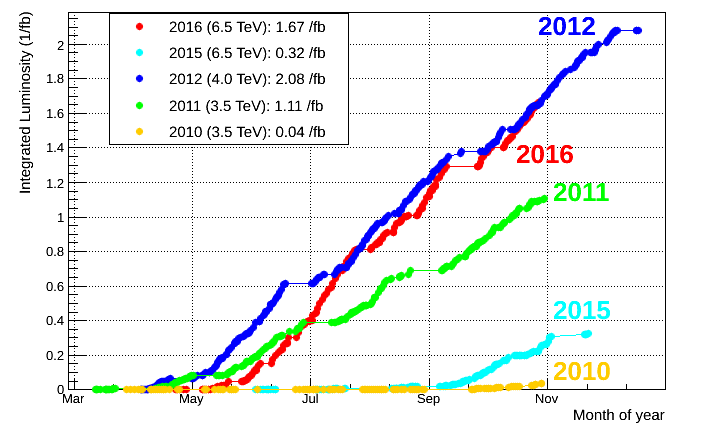
\includegraphics[ width=0.8\textwidth]{./Figs/LHC_LHCb/IntLumiRun1-2.png}
  \caption{Intergrated luminoscity collected by the LHCb experiment in each year of data taking. Source: LHCb.}
  \label{fig:LHCb_lumi}
\end{figure}


\begin{figure}[htb] 
  \centering    
  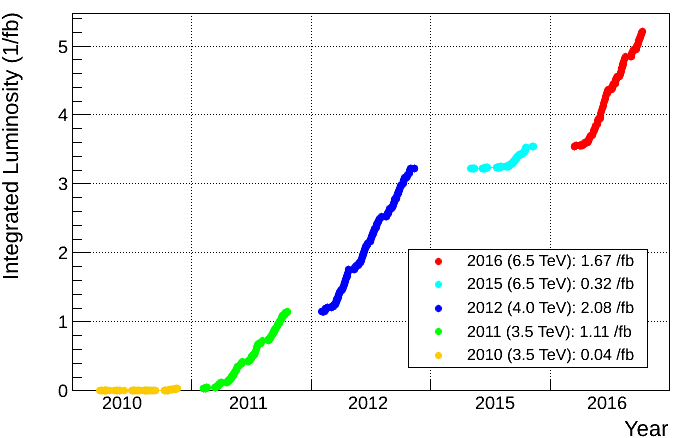
\includegraphics[ width=0.8\textwidth]{./Figs/LHC_LHCb/IntegratedLumiCumul.png}
  \caption{Cumulative intertrated luminoscity collected over data taking years at the LHCb experiment. Source: LHCb.}
  \label{fig:LHCb_lumi_cuml}
\end{figure}


